\subsection{Initialization}
\begin{frame}{Initialization}
  \begin{itemize}
    \item Expose all
    \begin{itemize}
      \item Global variables
      \item Global functions
      \item Classes
    \end{itemize}
    \pause
    \item Each are bound to corresponding proxy methods
    \item An object which members are the exposed features is beeing passed to node
  \end{itemize}
  \pause
  \begin{block}{Names}
    \begin{itemize}
      \item Functions and classes have the same name as in Root
      \item Global variables can be called using Get[Variable] and Set[Variable] methods
    \end{itemize}
  \end{block}
\end{frame}
\begin{frame}{rootJS init}
  \begin{columns}[T]
  \column{.1\textwidth}
    \begin{scriptsize}
      \only<1>{\vspace{6mm} $\rightarrow$}
      \only<2>{\vspace{15mm} $\rightarrow$}
      \only<3>{\vspace{24mm} $\rightarrow$}
      \only<4>{\vspace{41mm} $\rightarrow$}
      \only<5>{\vspace{52mm} $\rightarrow$}
      \only<6>{\vspace{64mm} $\rightarrow$}
    \end{scriptsize}
  \column{.9\textwidth}
    \only<1>{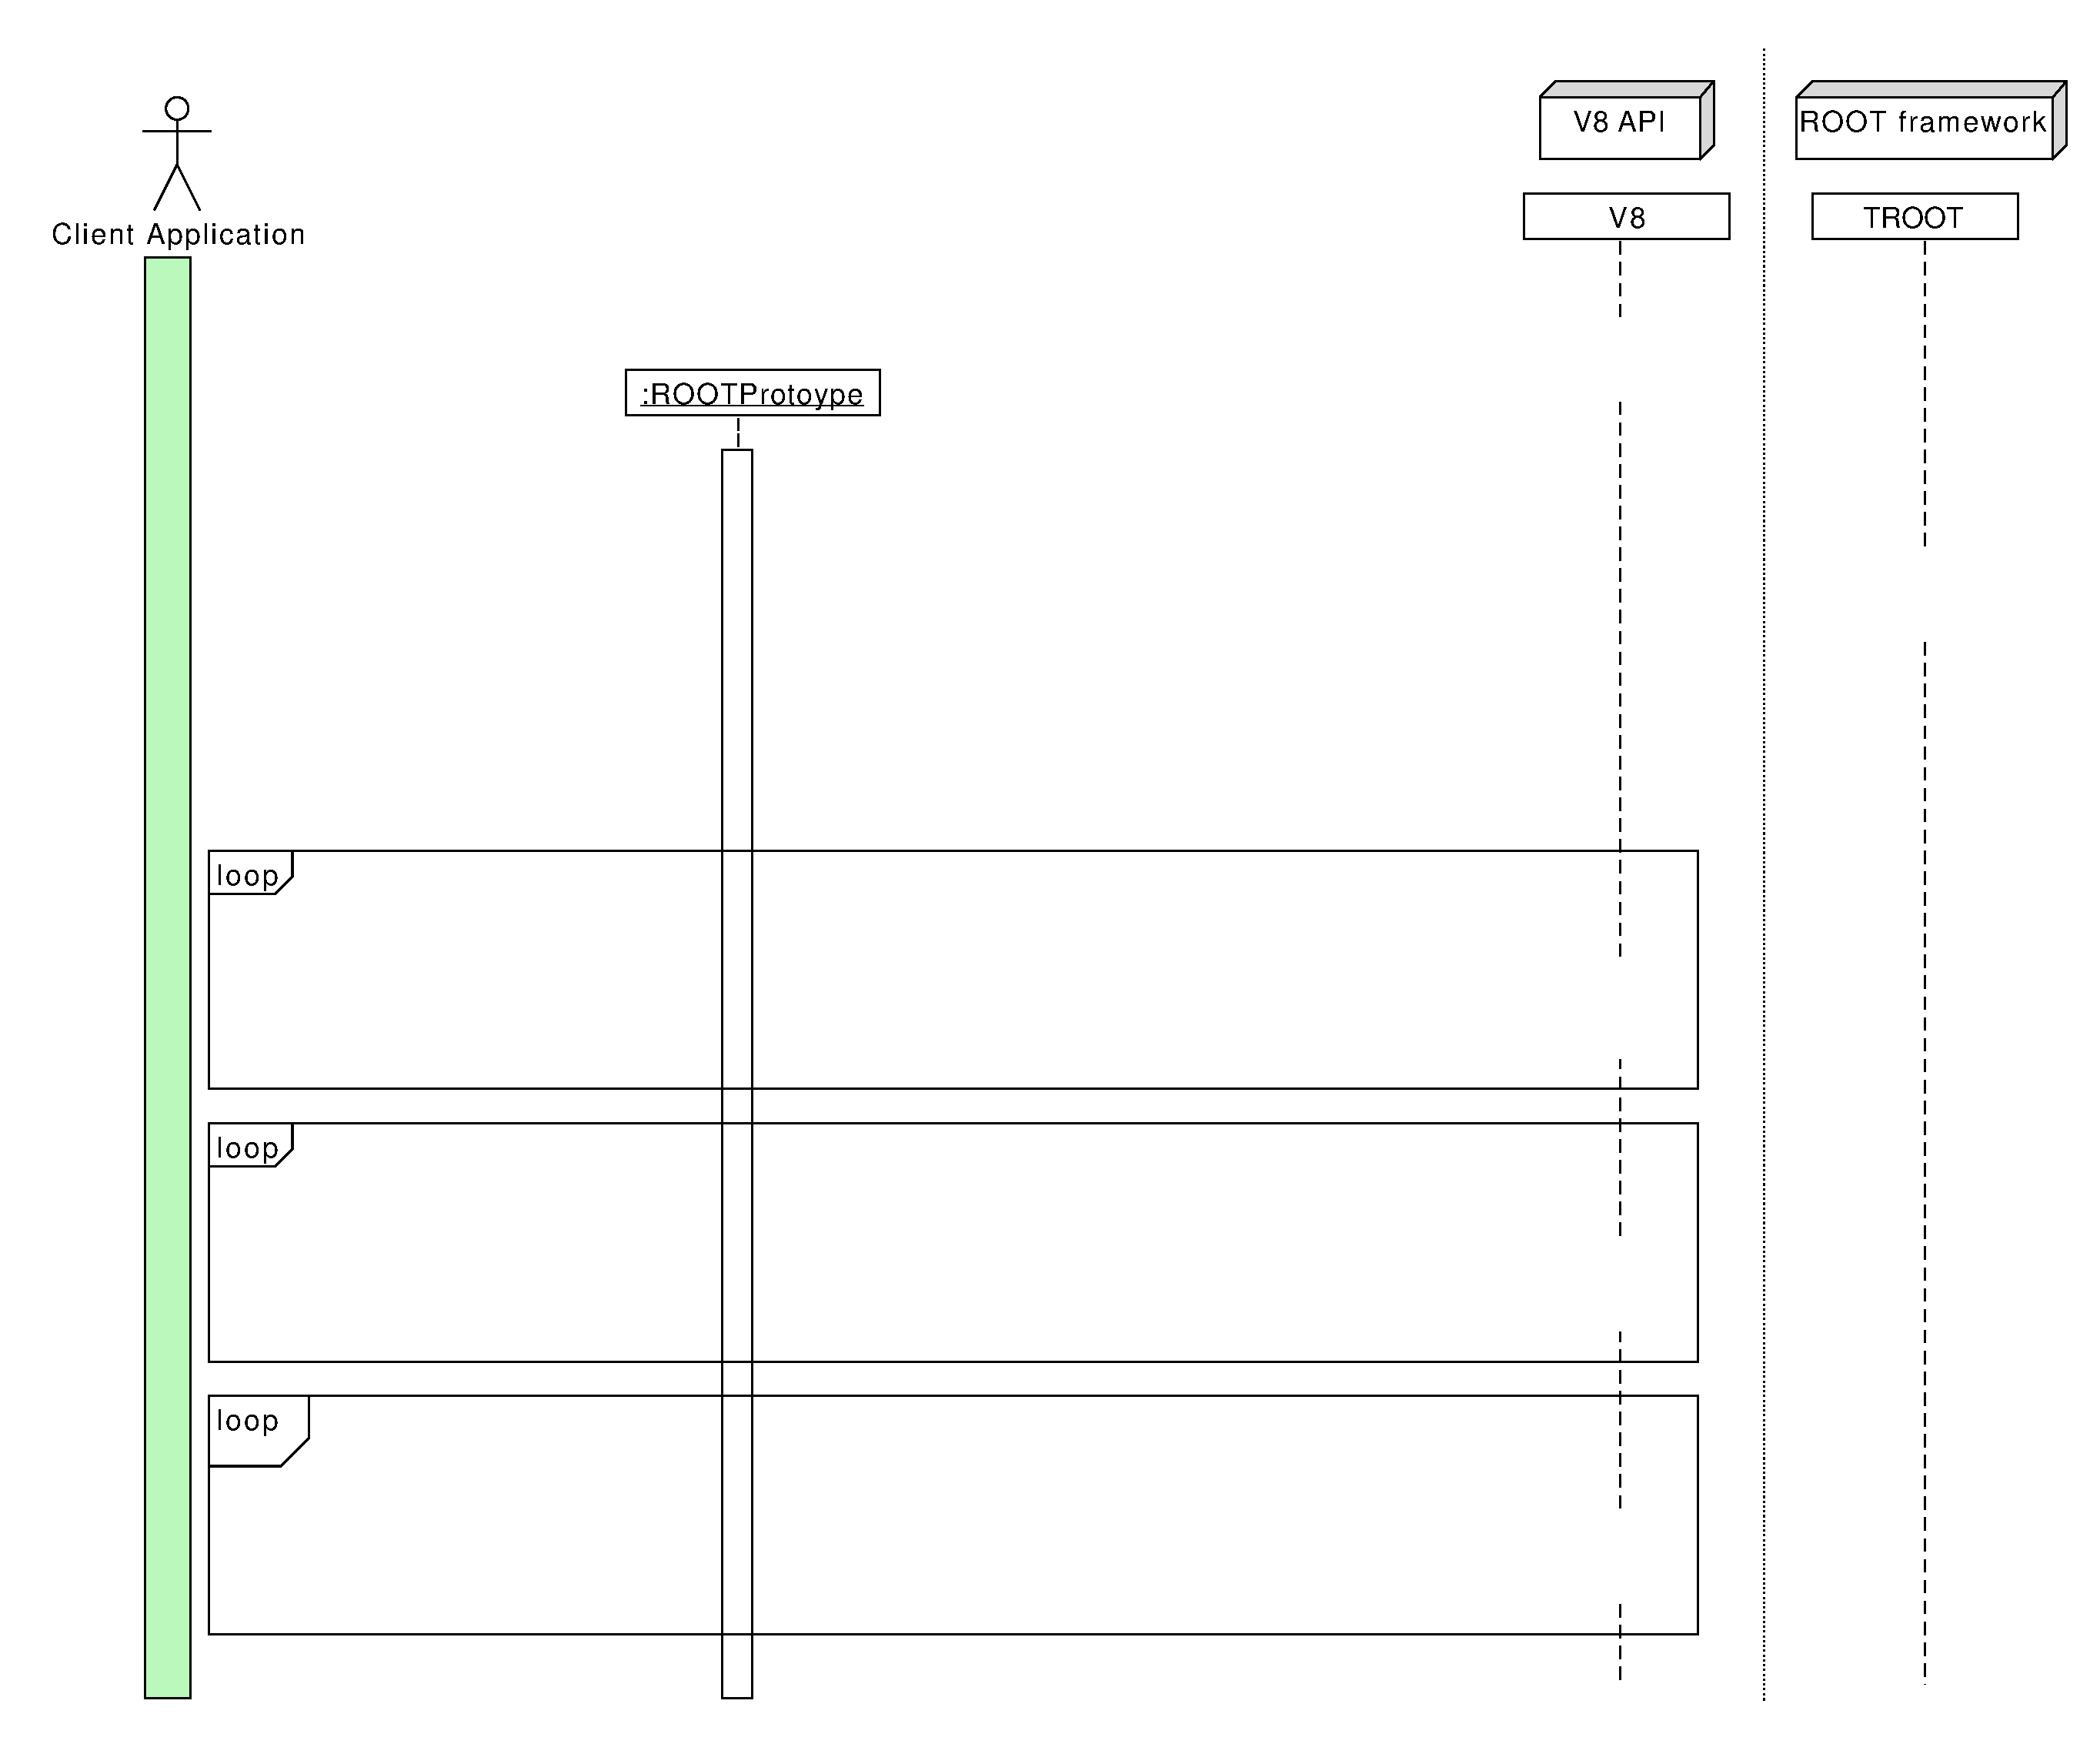
\includegraphics[width=\linewidth, height=.85\textheight, keepaspectratio]{./resources/initialize/initialize_h1.pdf}}
    \only<2>{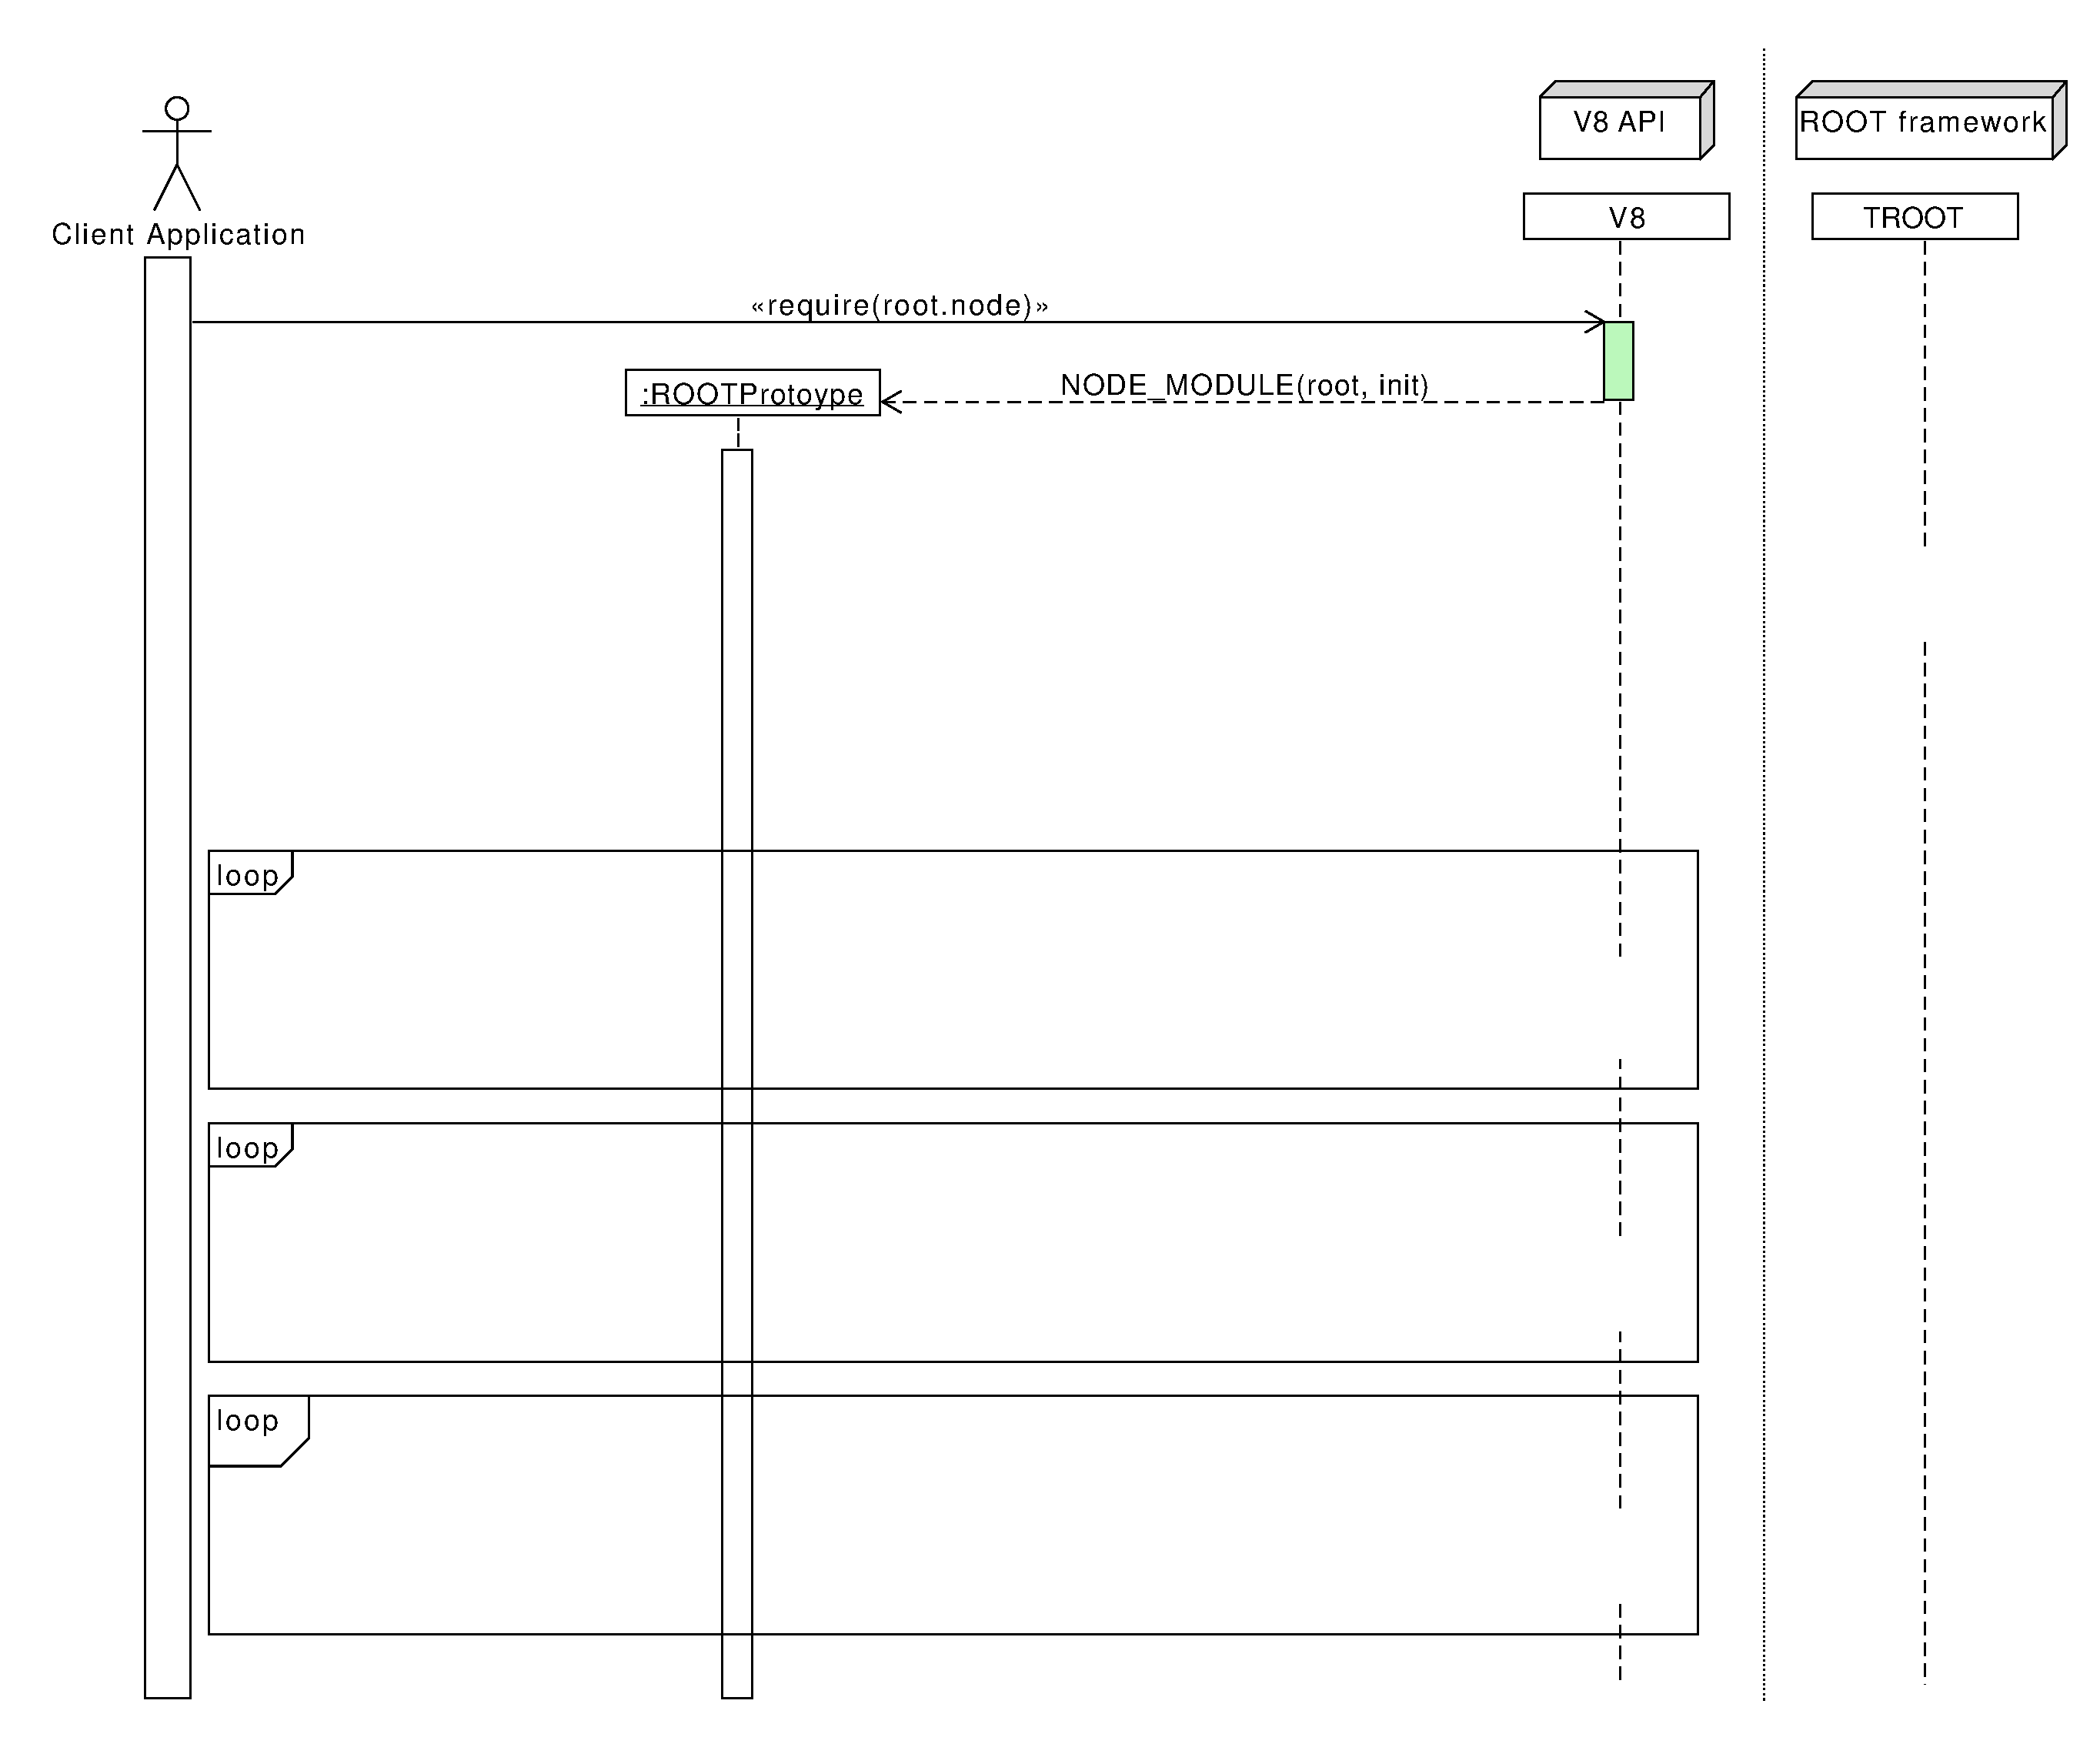
\includegraphics[width=\linewidth, height=.85\textheight, keepaspectratio]{./resources/initialize/initialize_h2.pdf}}
    \only<3>{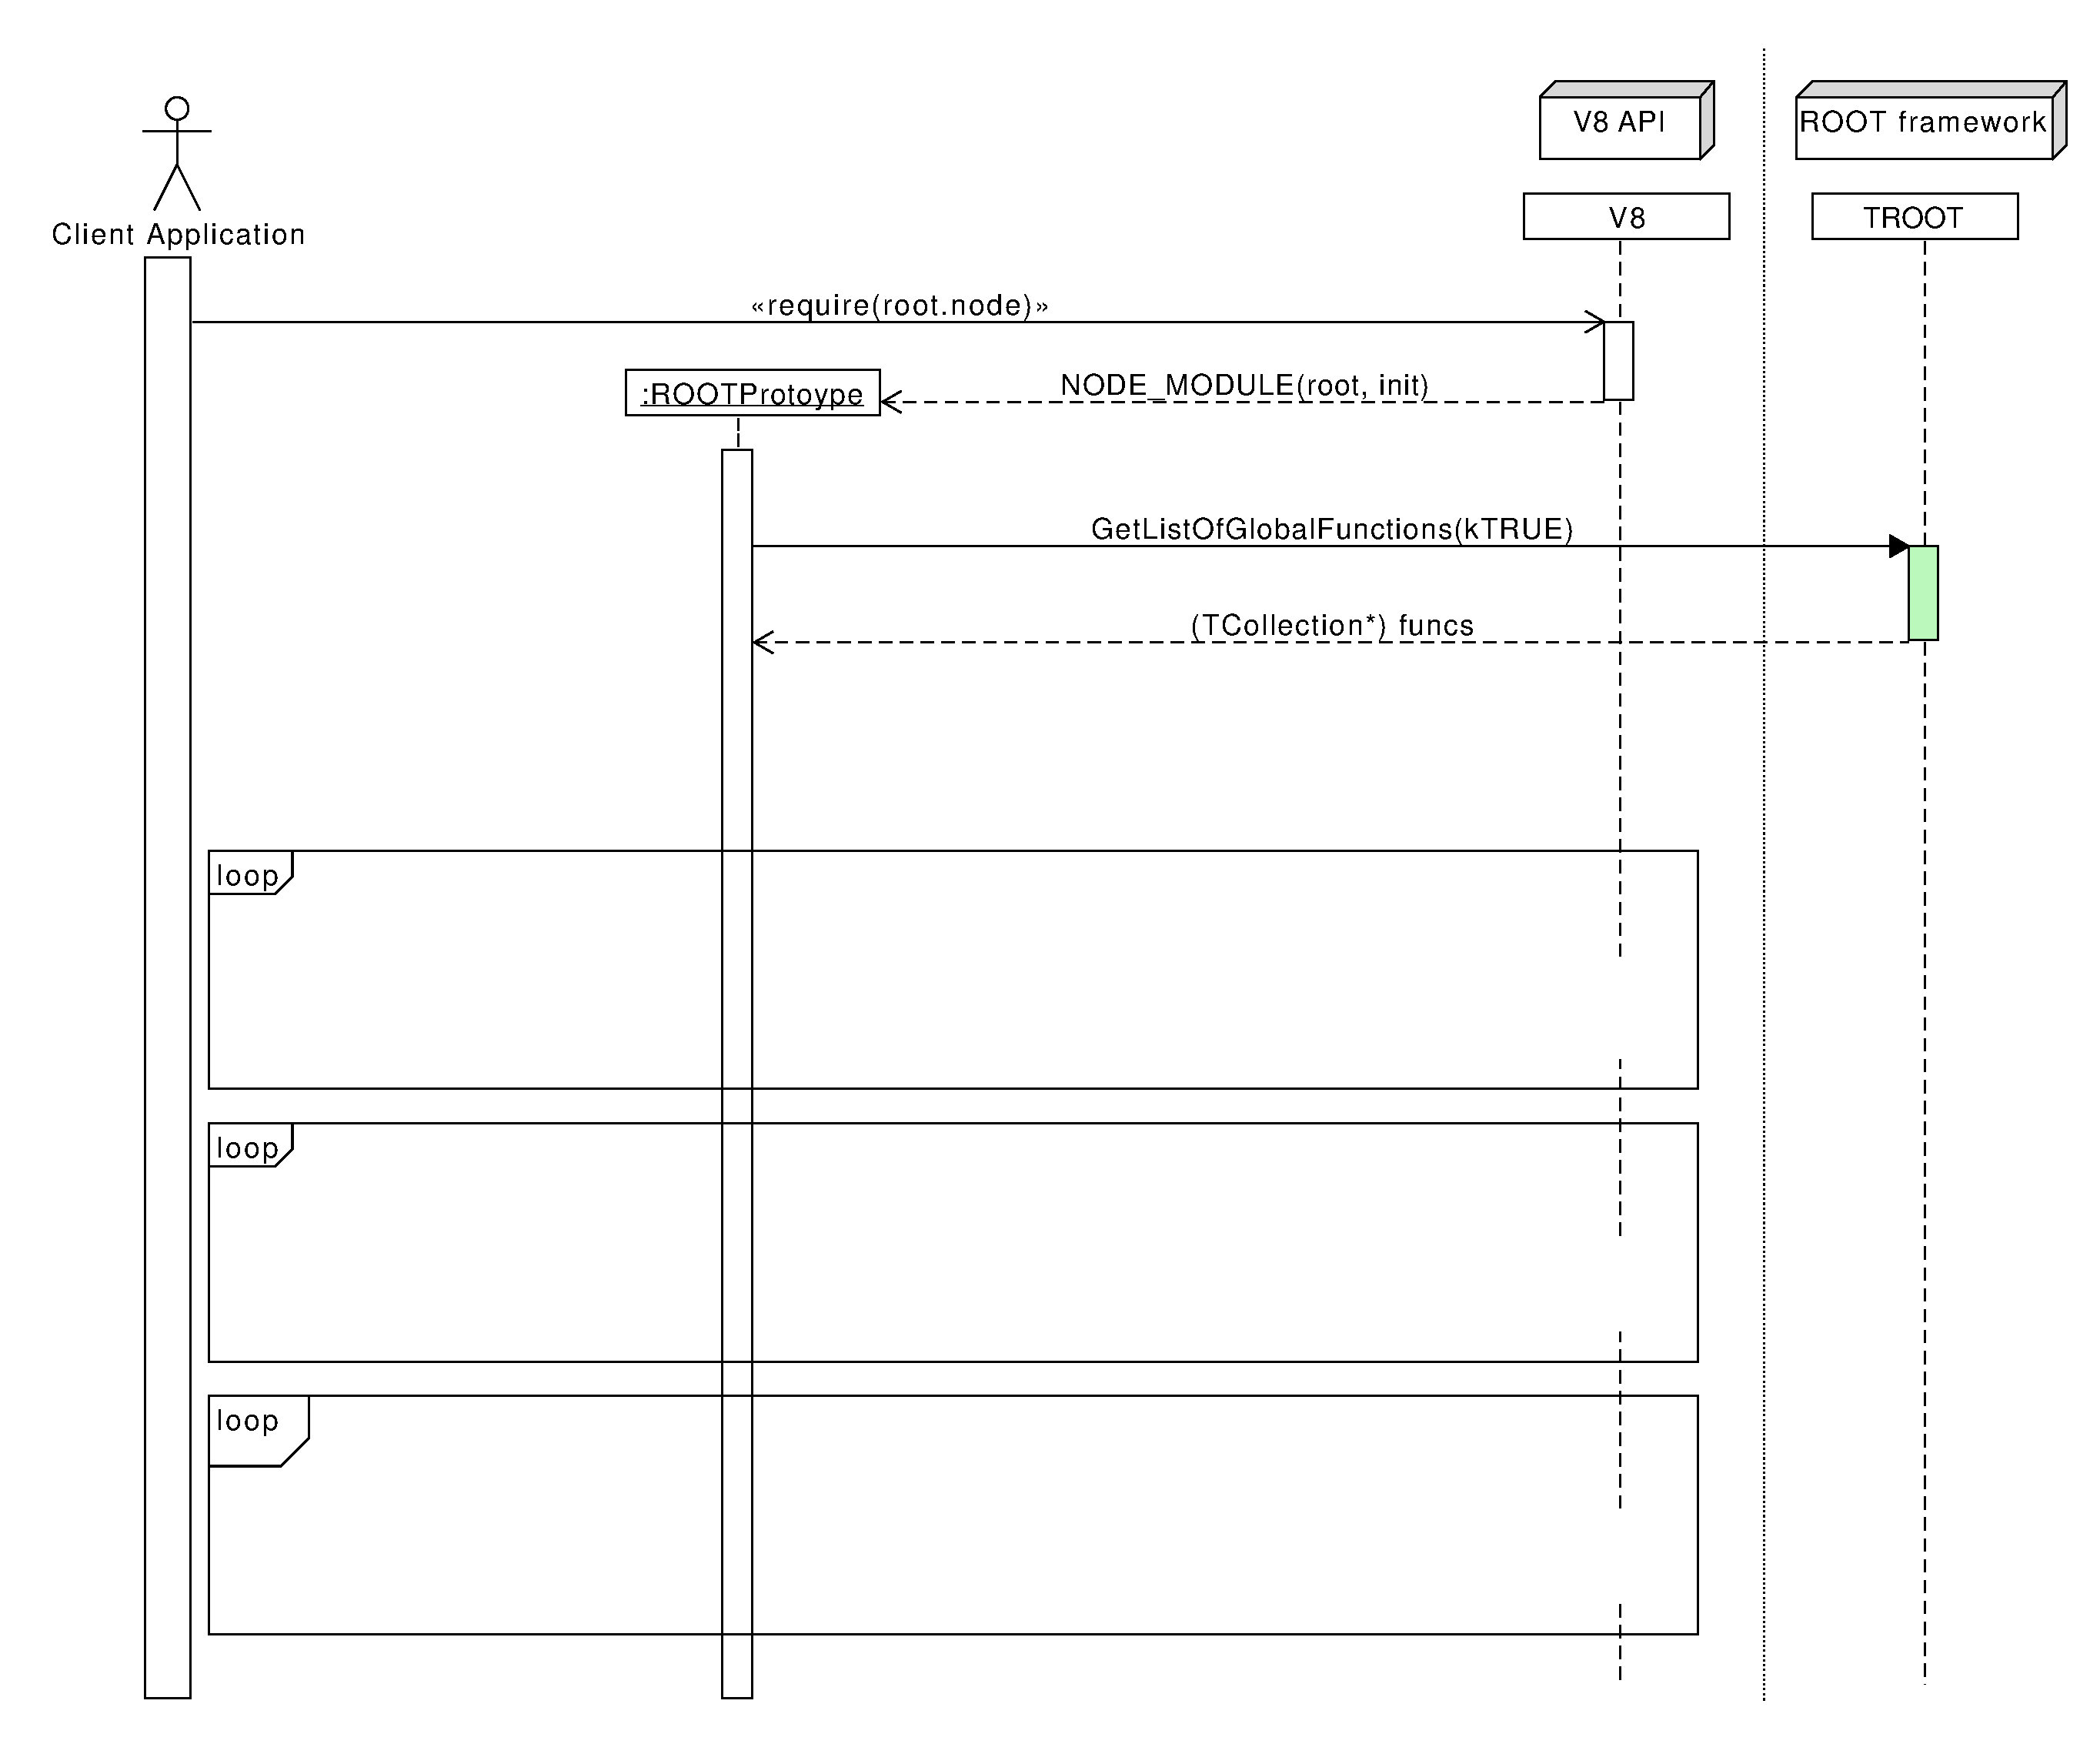
\includegraphics[width=\linewidth, height=.85\textheight, keepaspectratio]{./resources/initialize/initialize_h3.pdf}}
    \only<4>{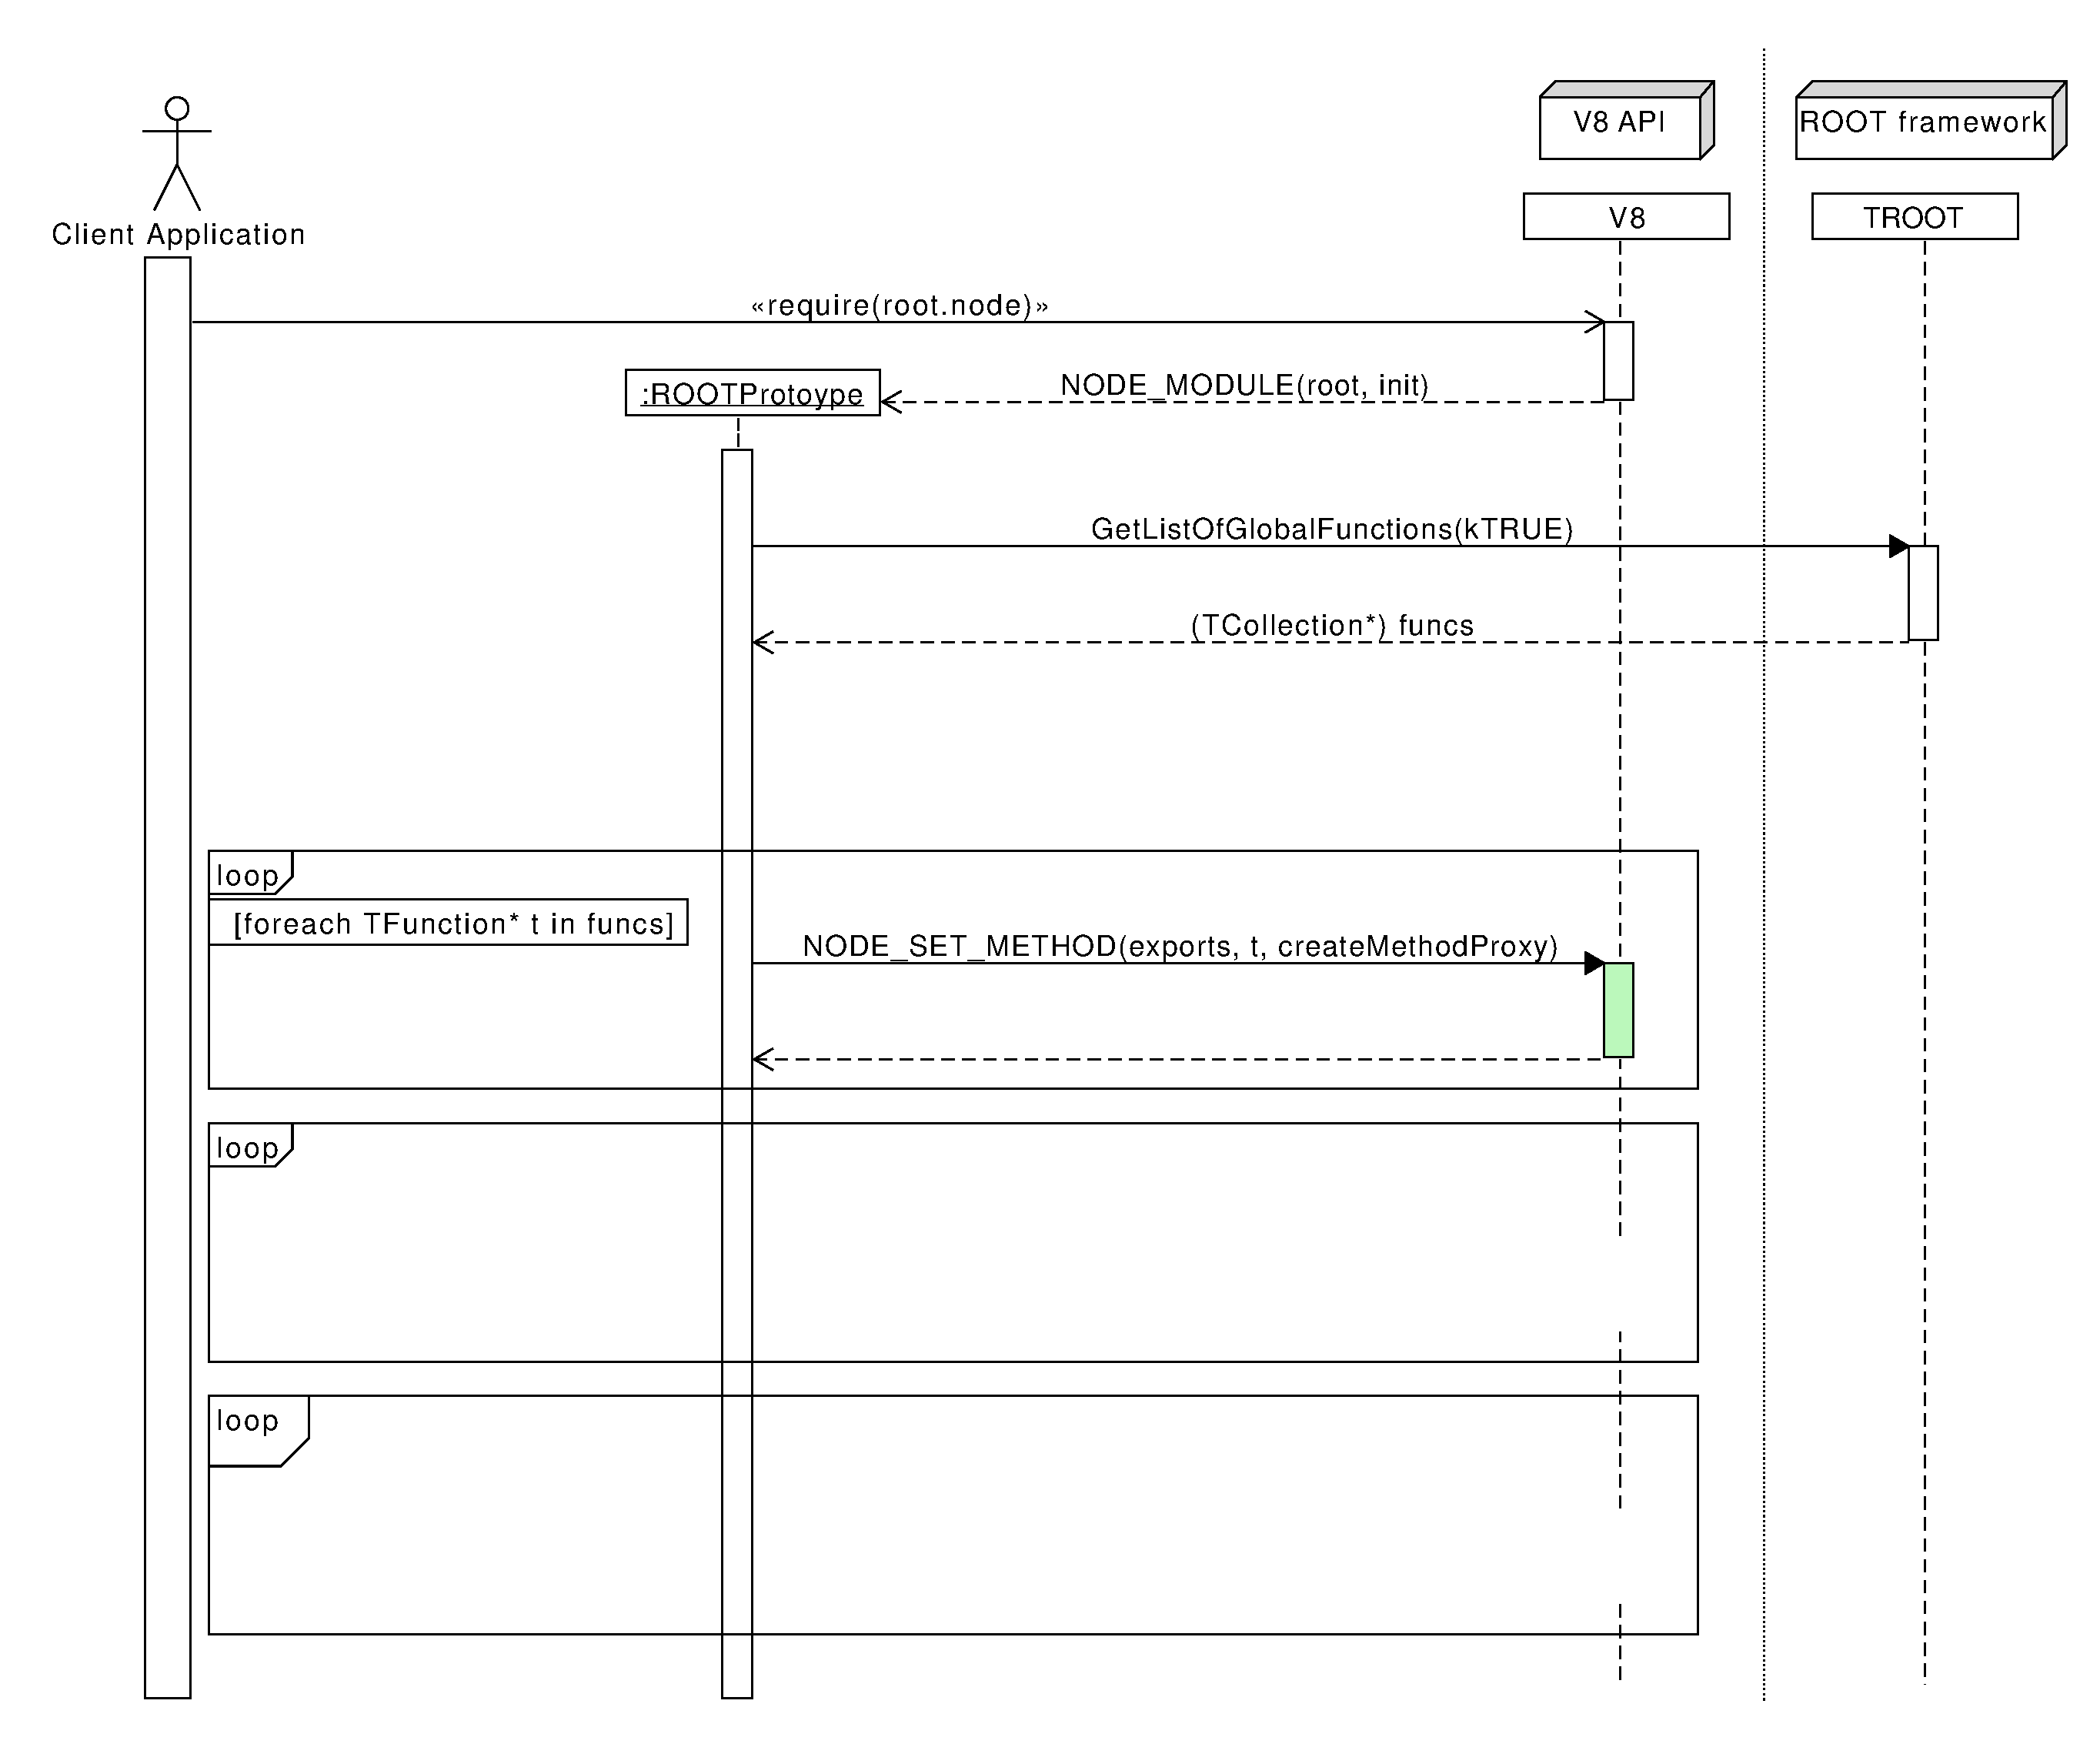
\includegraphics[width=\linewidth, height=.85\textheight, keepaspectratio]{./resources/initialize/initialize_h4.pdf}}
    \only<5>{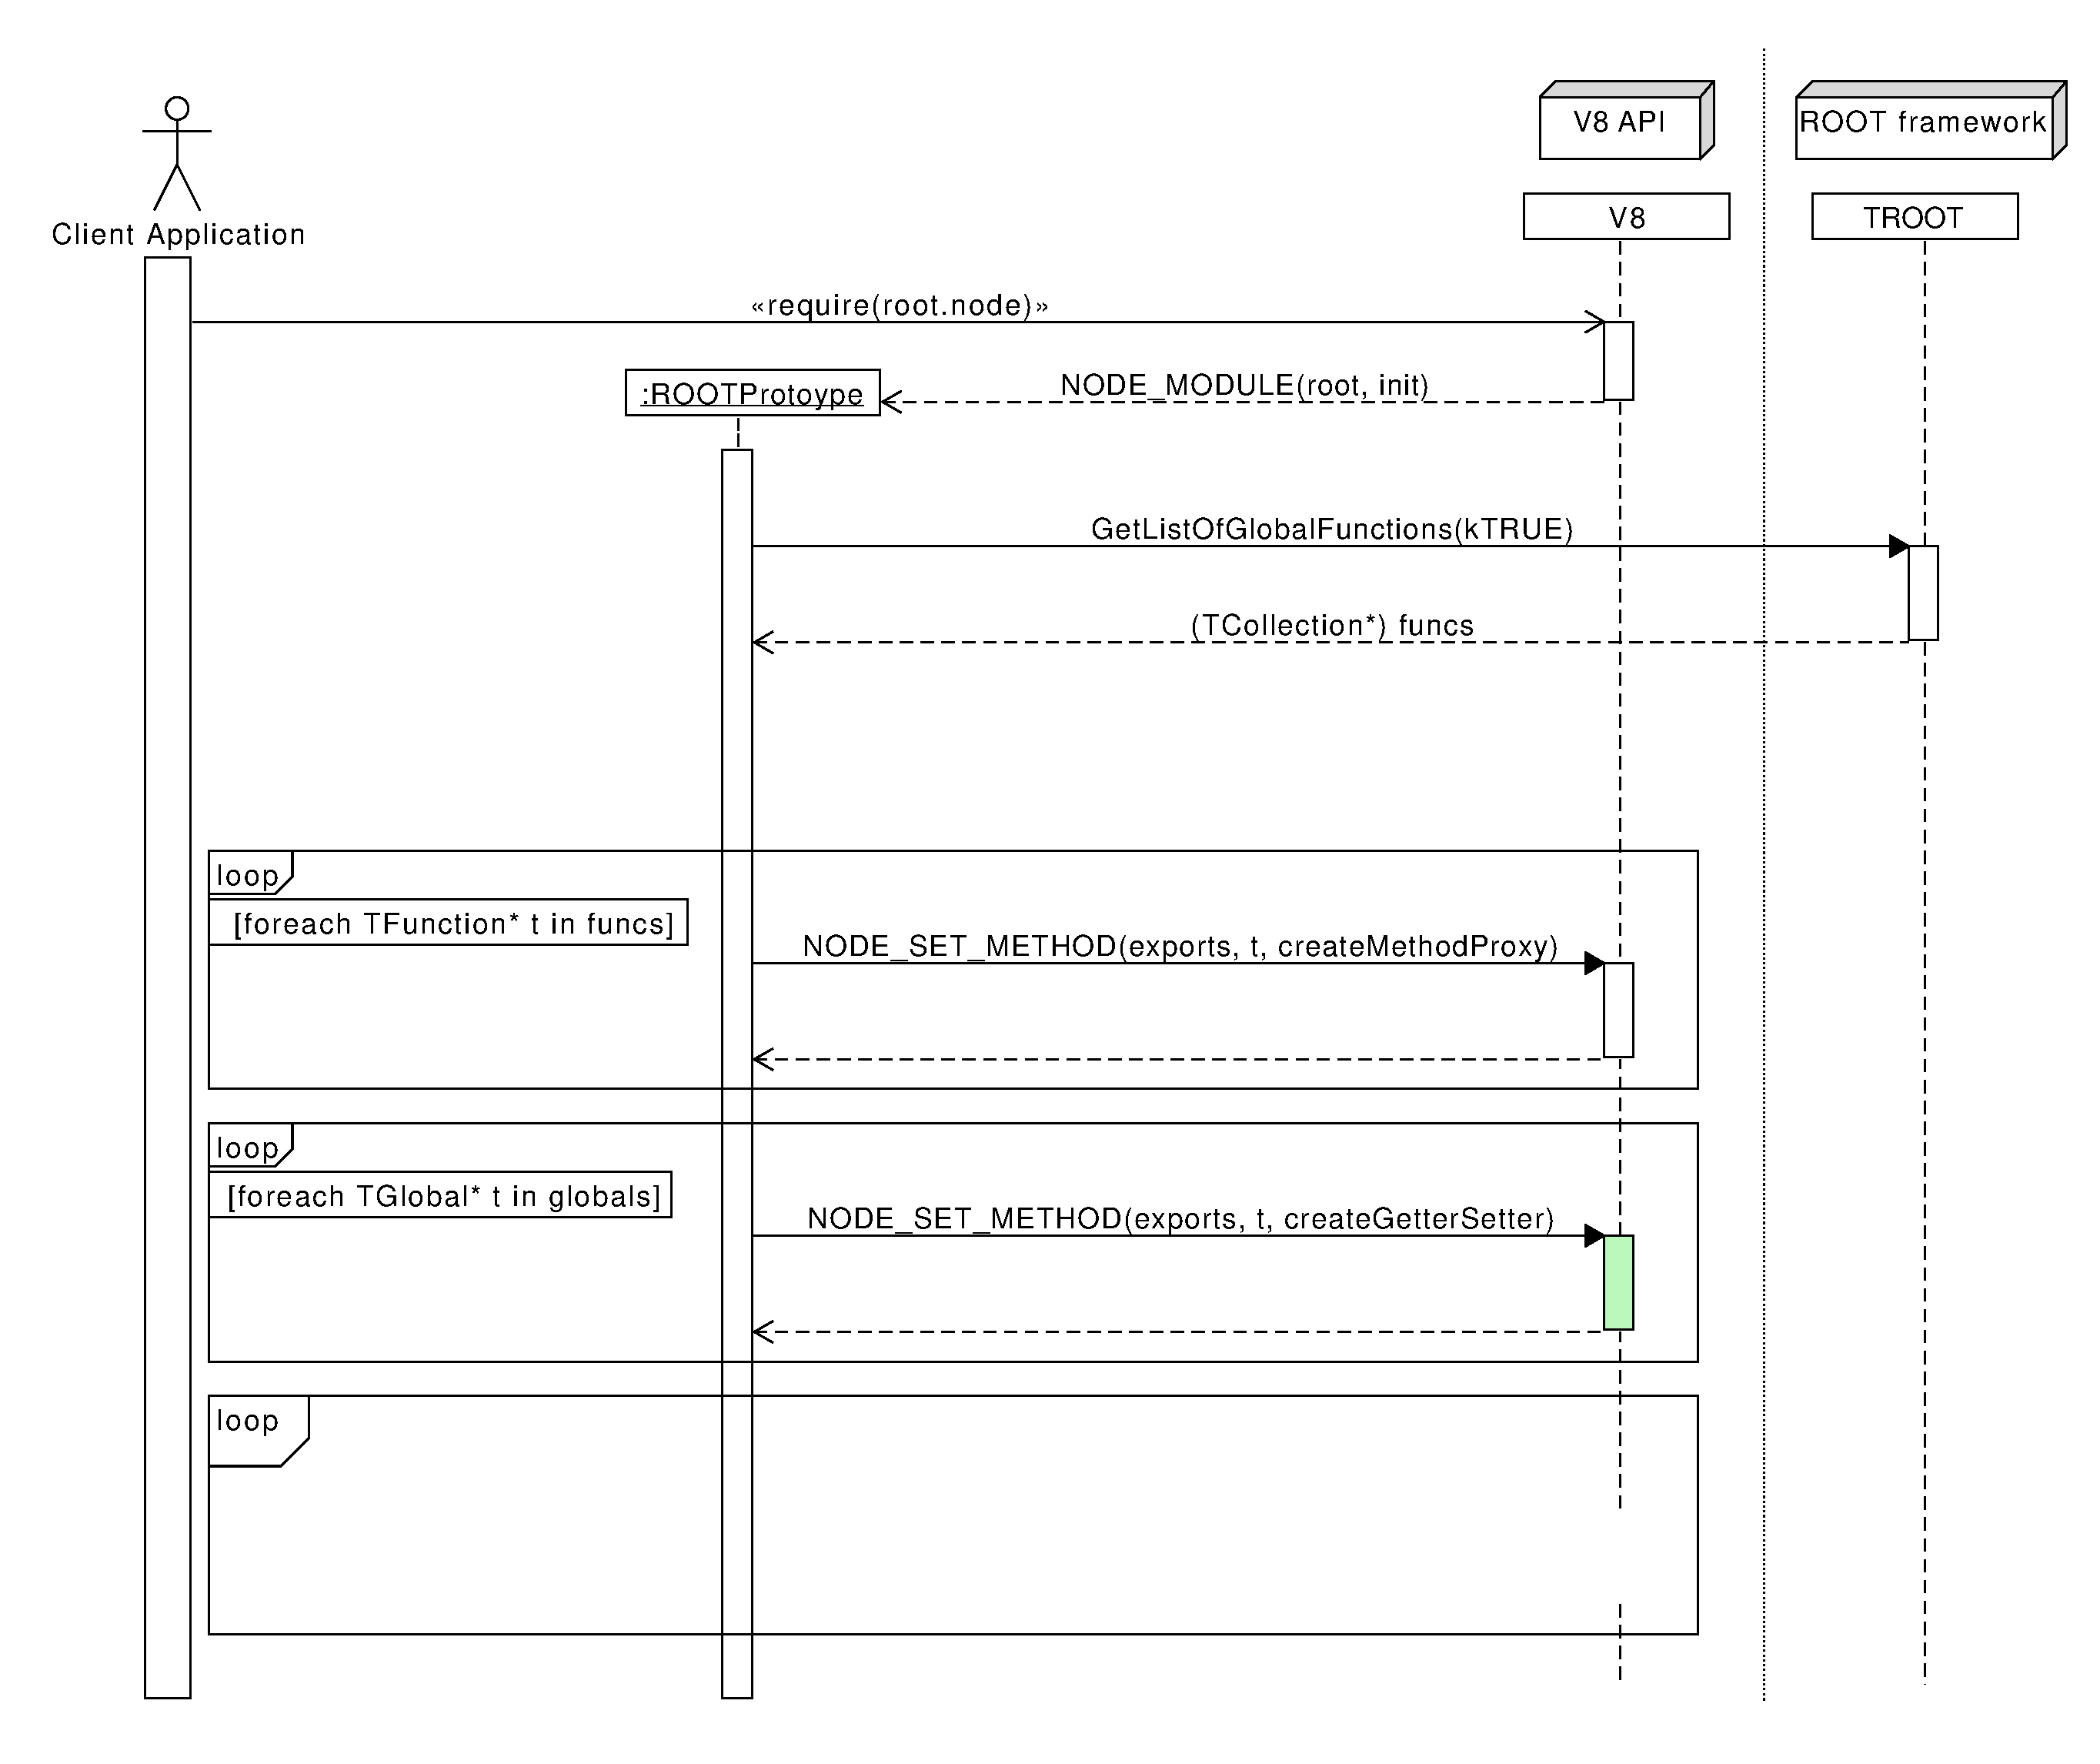
\includegraphics[width=\linewidth, height=.85\textheight, keepaspectratio]{./resources/initialize/initialize_h5.pdf}}
    \only<6>{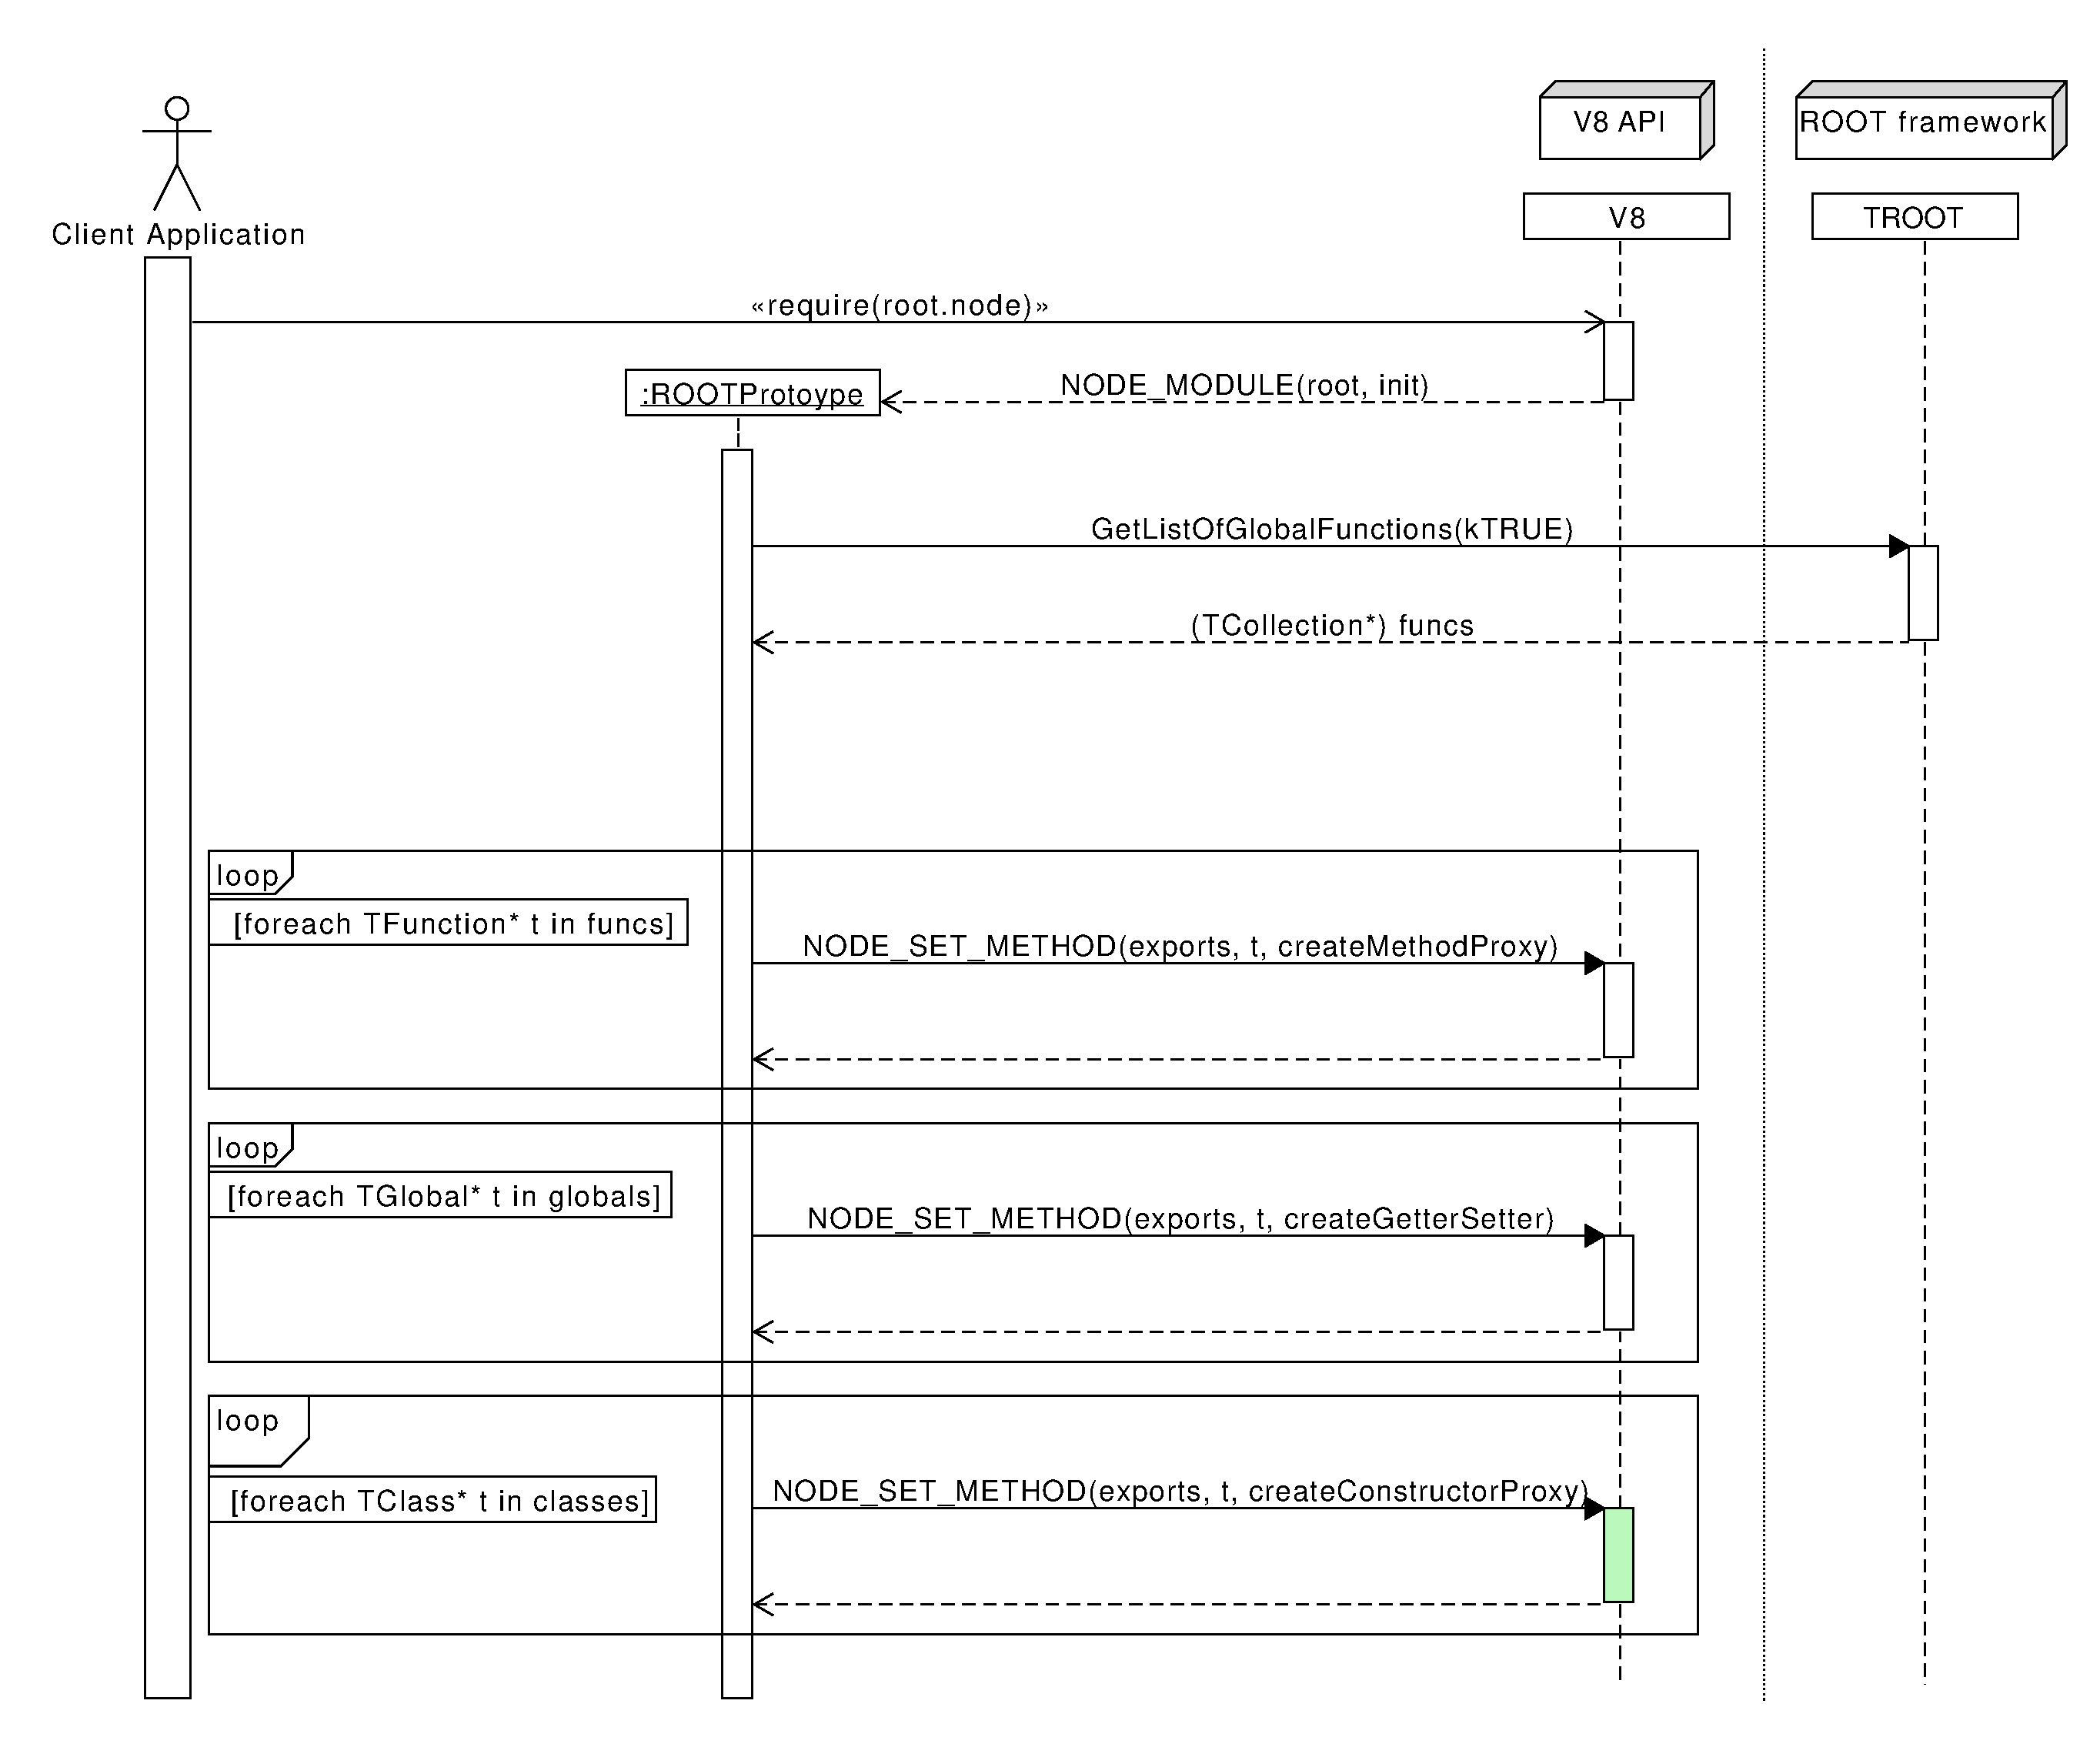
\includegraphics[width=\linewidth, height=.85\textheight, keepaspectratio]{./resources/initialize/initialize_h6.pdf}}
    \only<7>{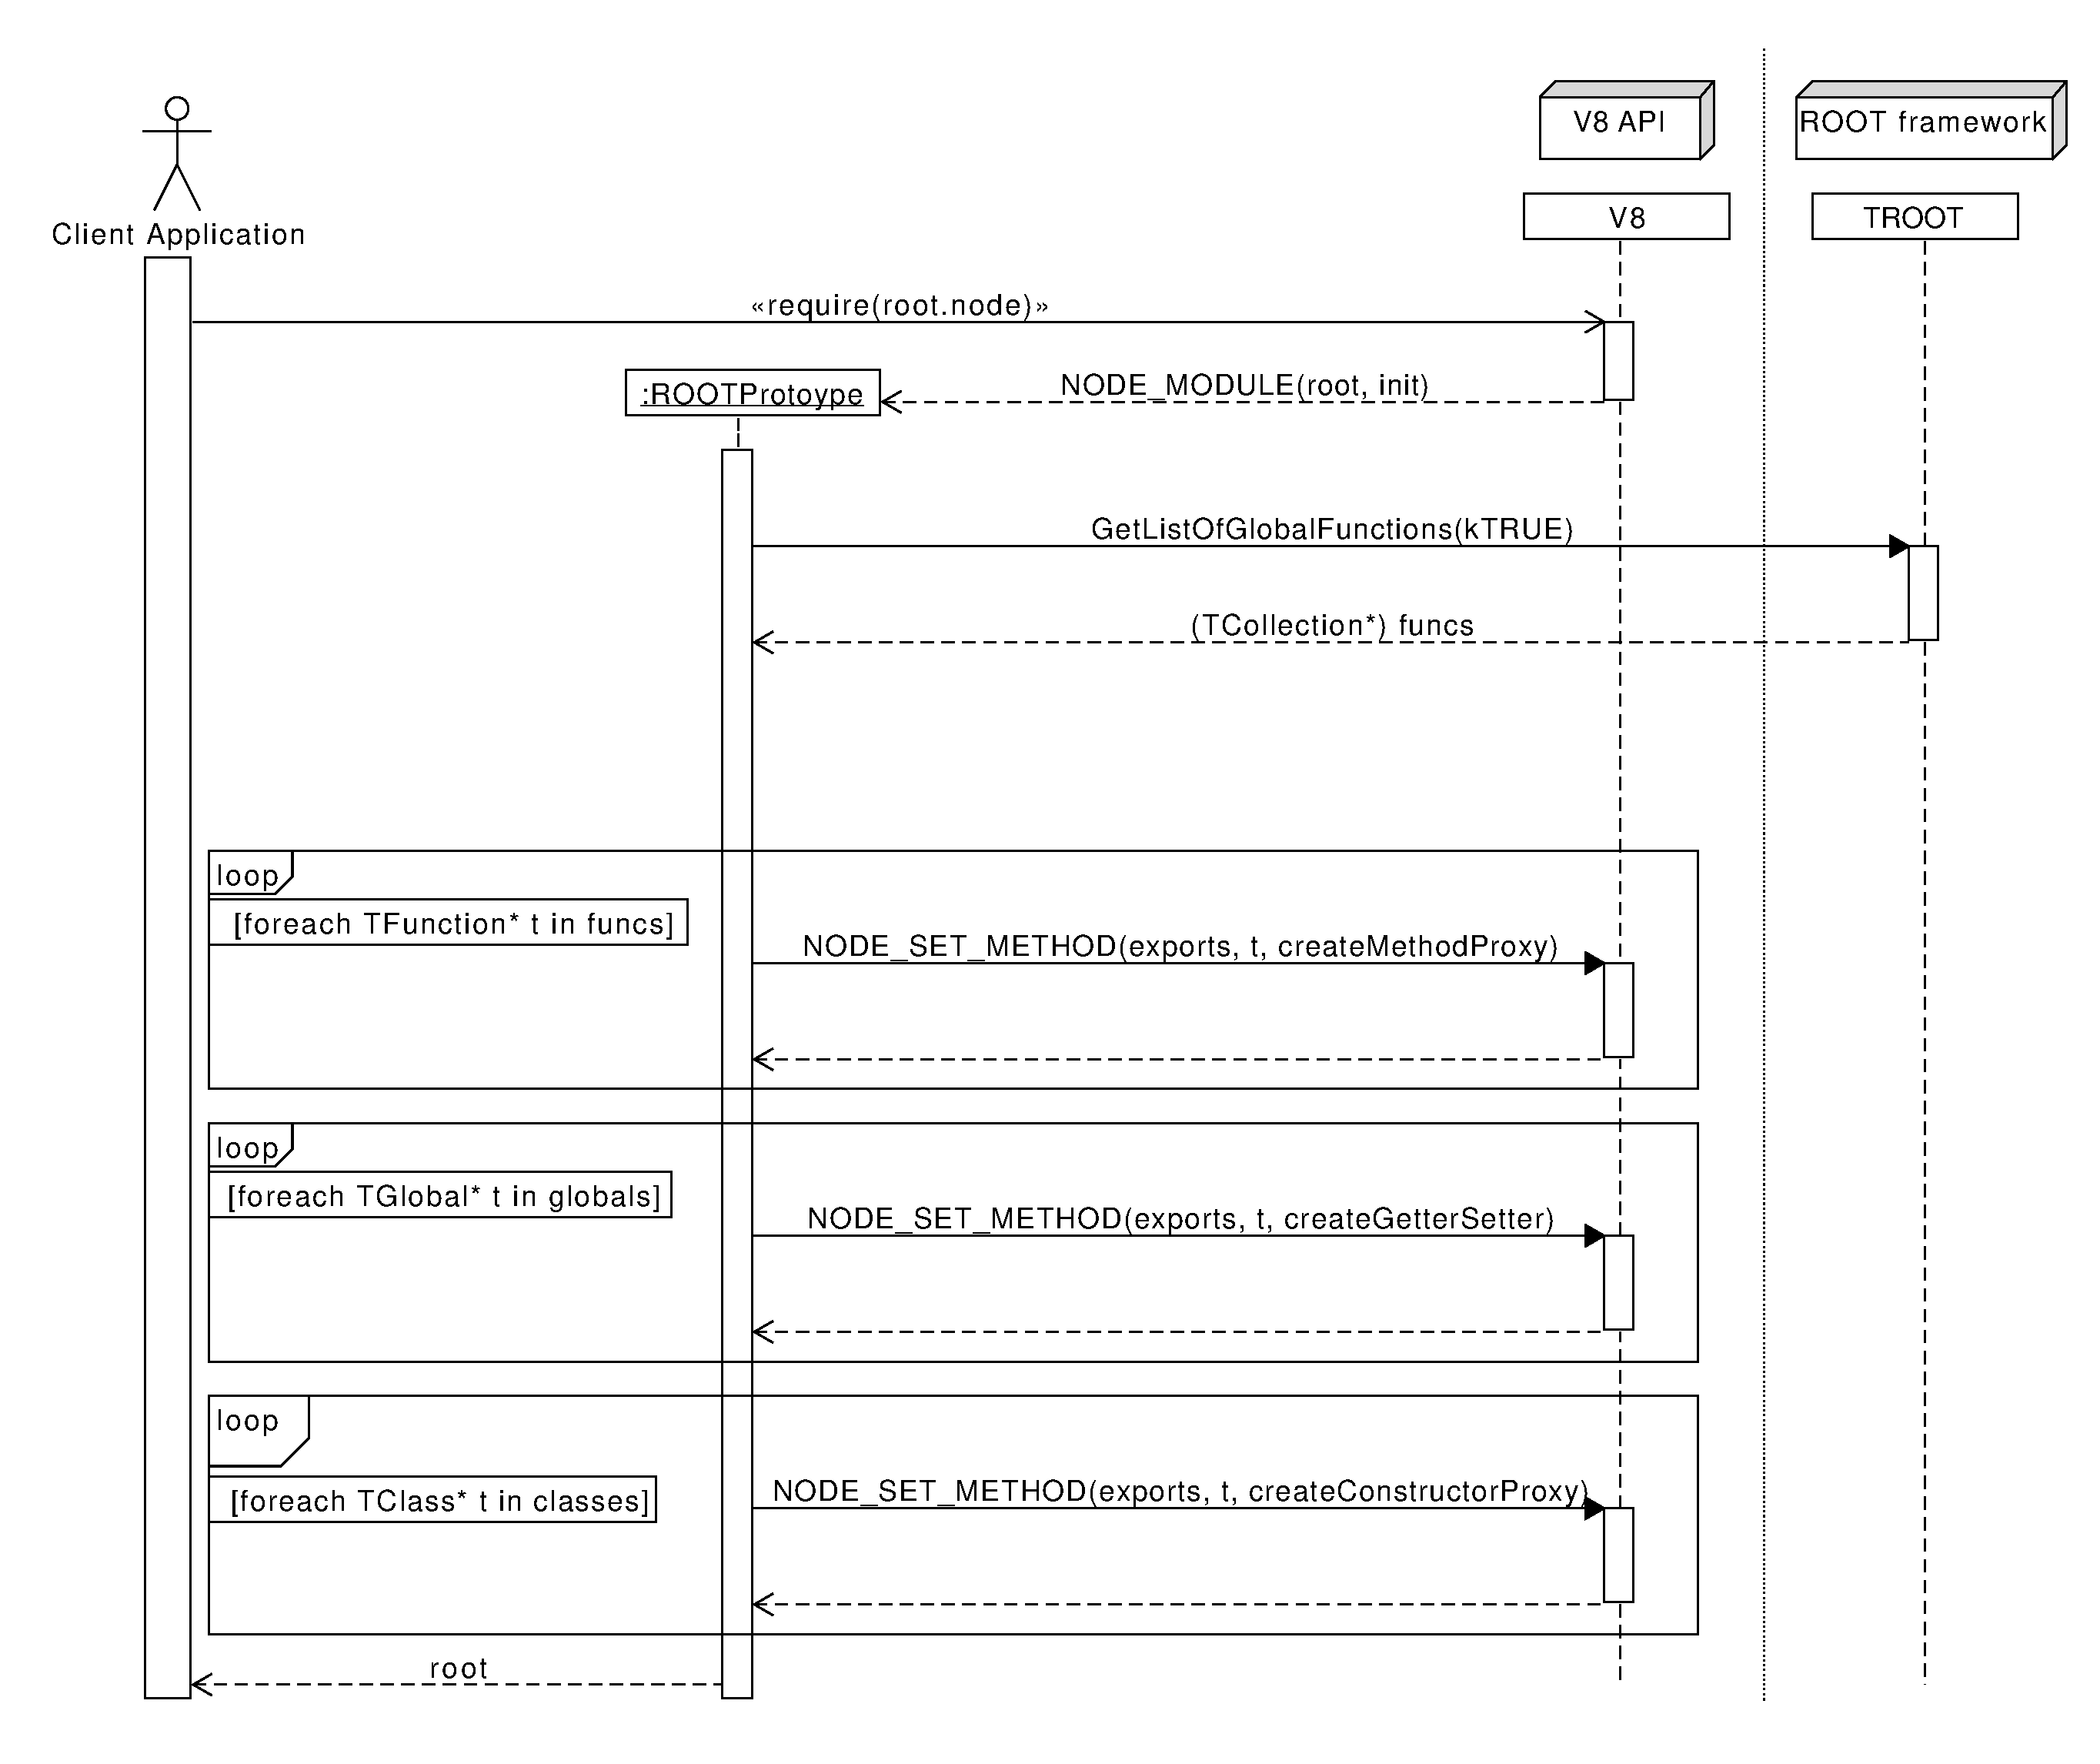
\includegraphics[width=\linewidth, height=.85\textheight, keepaspectratio]{./resources/initialize/initialize_h0.pdf}}
 \end{columns}
\end{frame}


\subsection{Call a feature}
\begin{frame}{Call a feature}
  \begin{itemize}
    \item All features in node are mapped to a proxy method that will be called
    \pause
    \item The proxy method will eventually call a root function and pass the result to our ObjectFactory
    \pause
    \item By looking at the object type an corresponding v8::Handle will be generated and returned to node
    \begin{itemize}
      \item If the result is an object this will be done recursively
    \end{itemize}
  \end{itemize}
\end{frame}
\begin{frame}{proxied file access}
  \begin{figure}[htb]
    \centering
      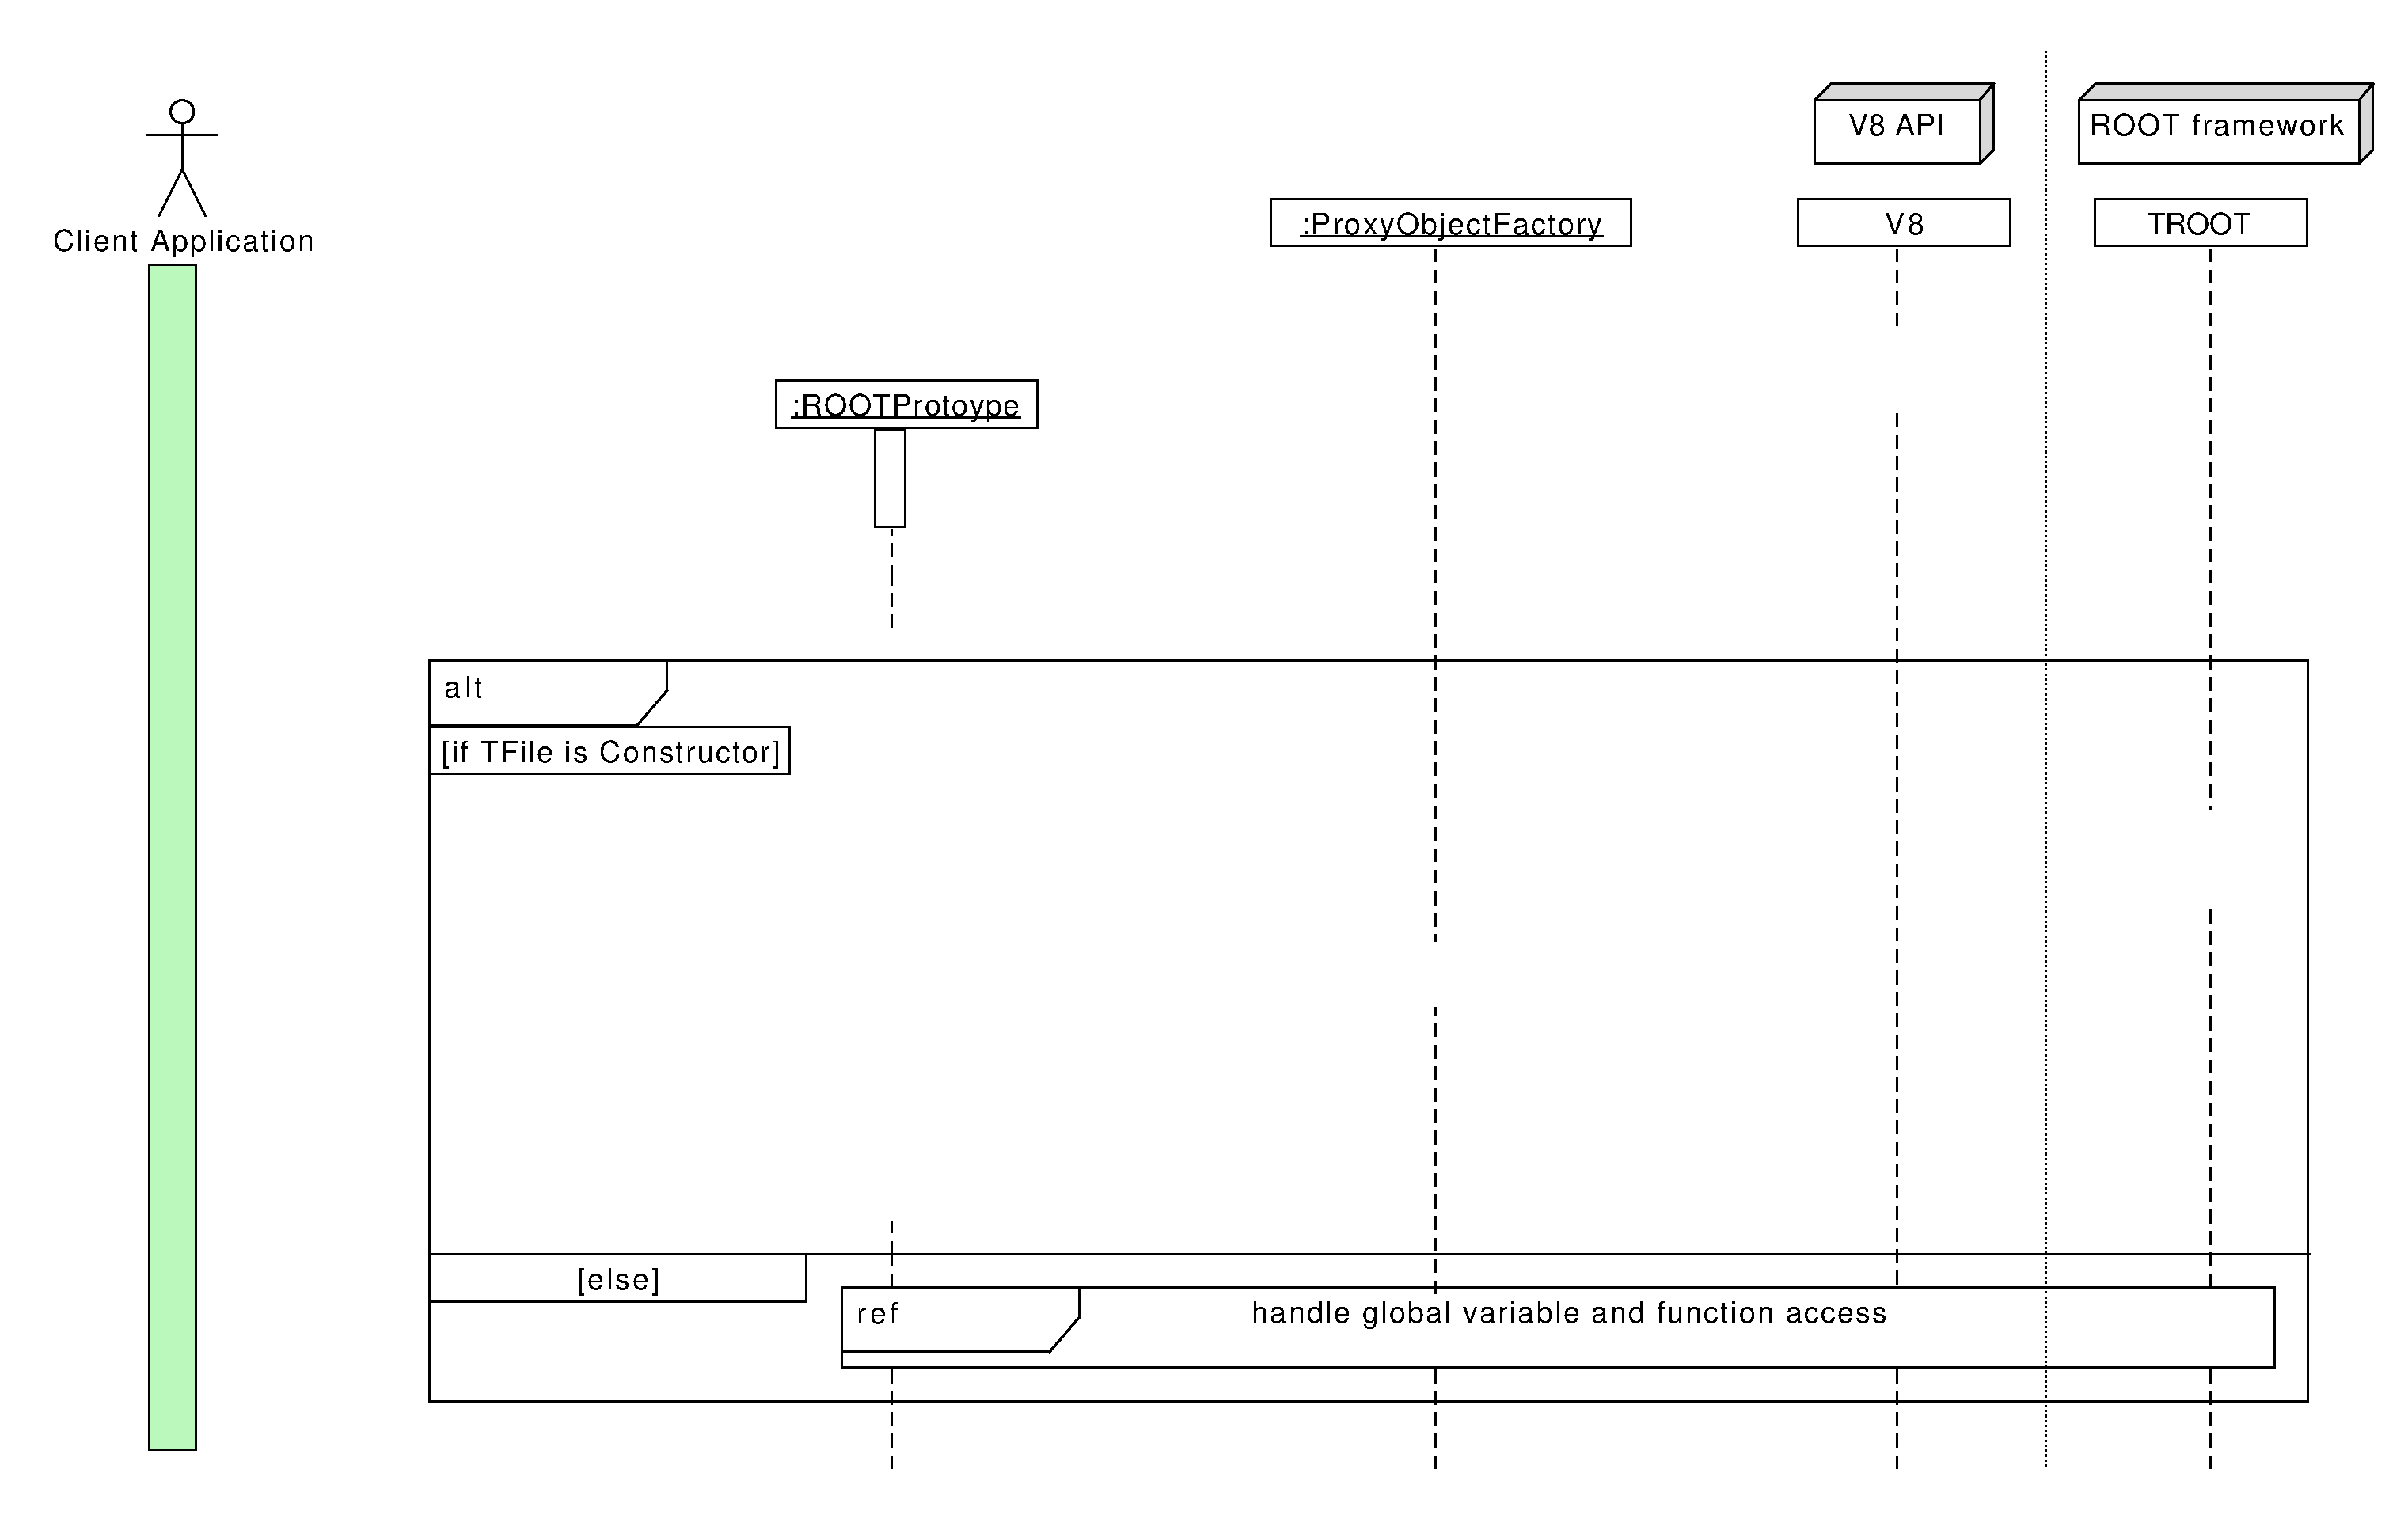
\includegraphics[width=\textwidth, height=.85\textheight, keepaspectratio]{./resources/proxycall/fileOpen_h1.pdf}
  \end{figure}
\end{frame}

\begin{frame}{proxied file access}
  \begin{figure}[htb]
    \centering
      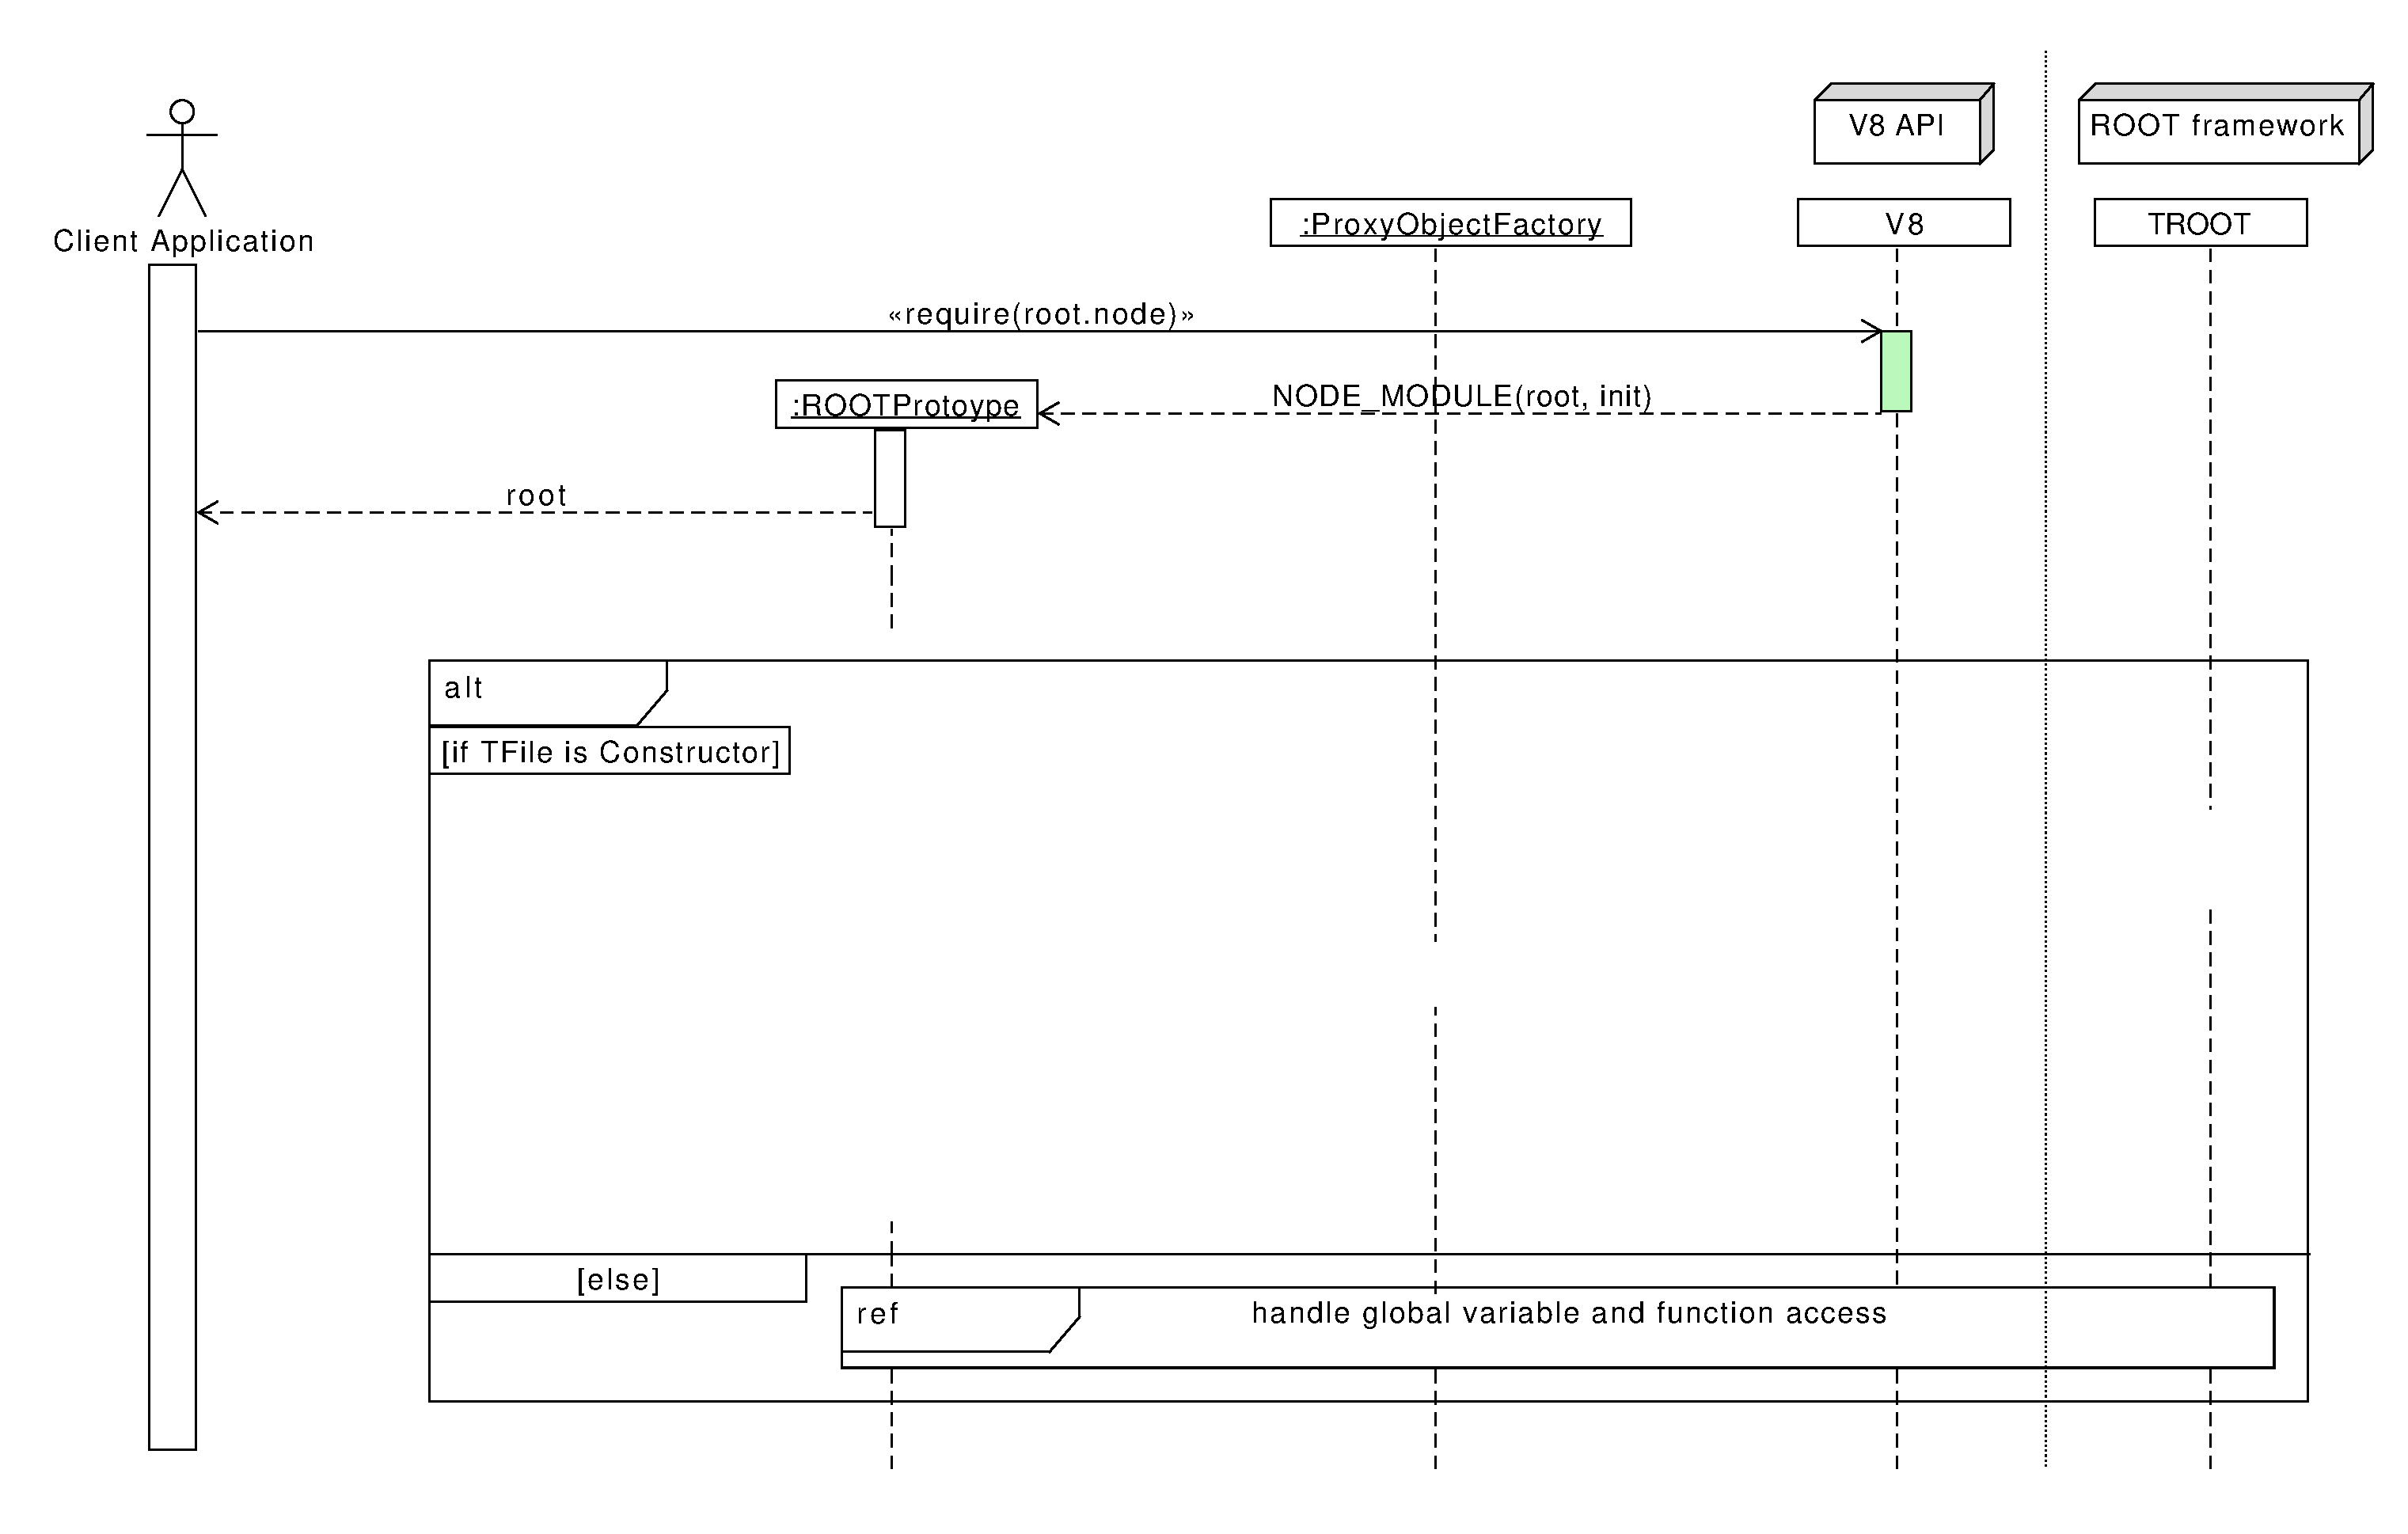
\includegraphics[width=\textwidth, height=.85\textheight, keepaspectratio]{./resources/proxycall/fileOpen_h2.pdf}
  \end{figure}
\end{frame}

\begin{frame}{proxied file access}
  \begin{figure}[htb]
    \centering
      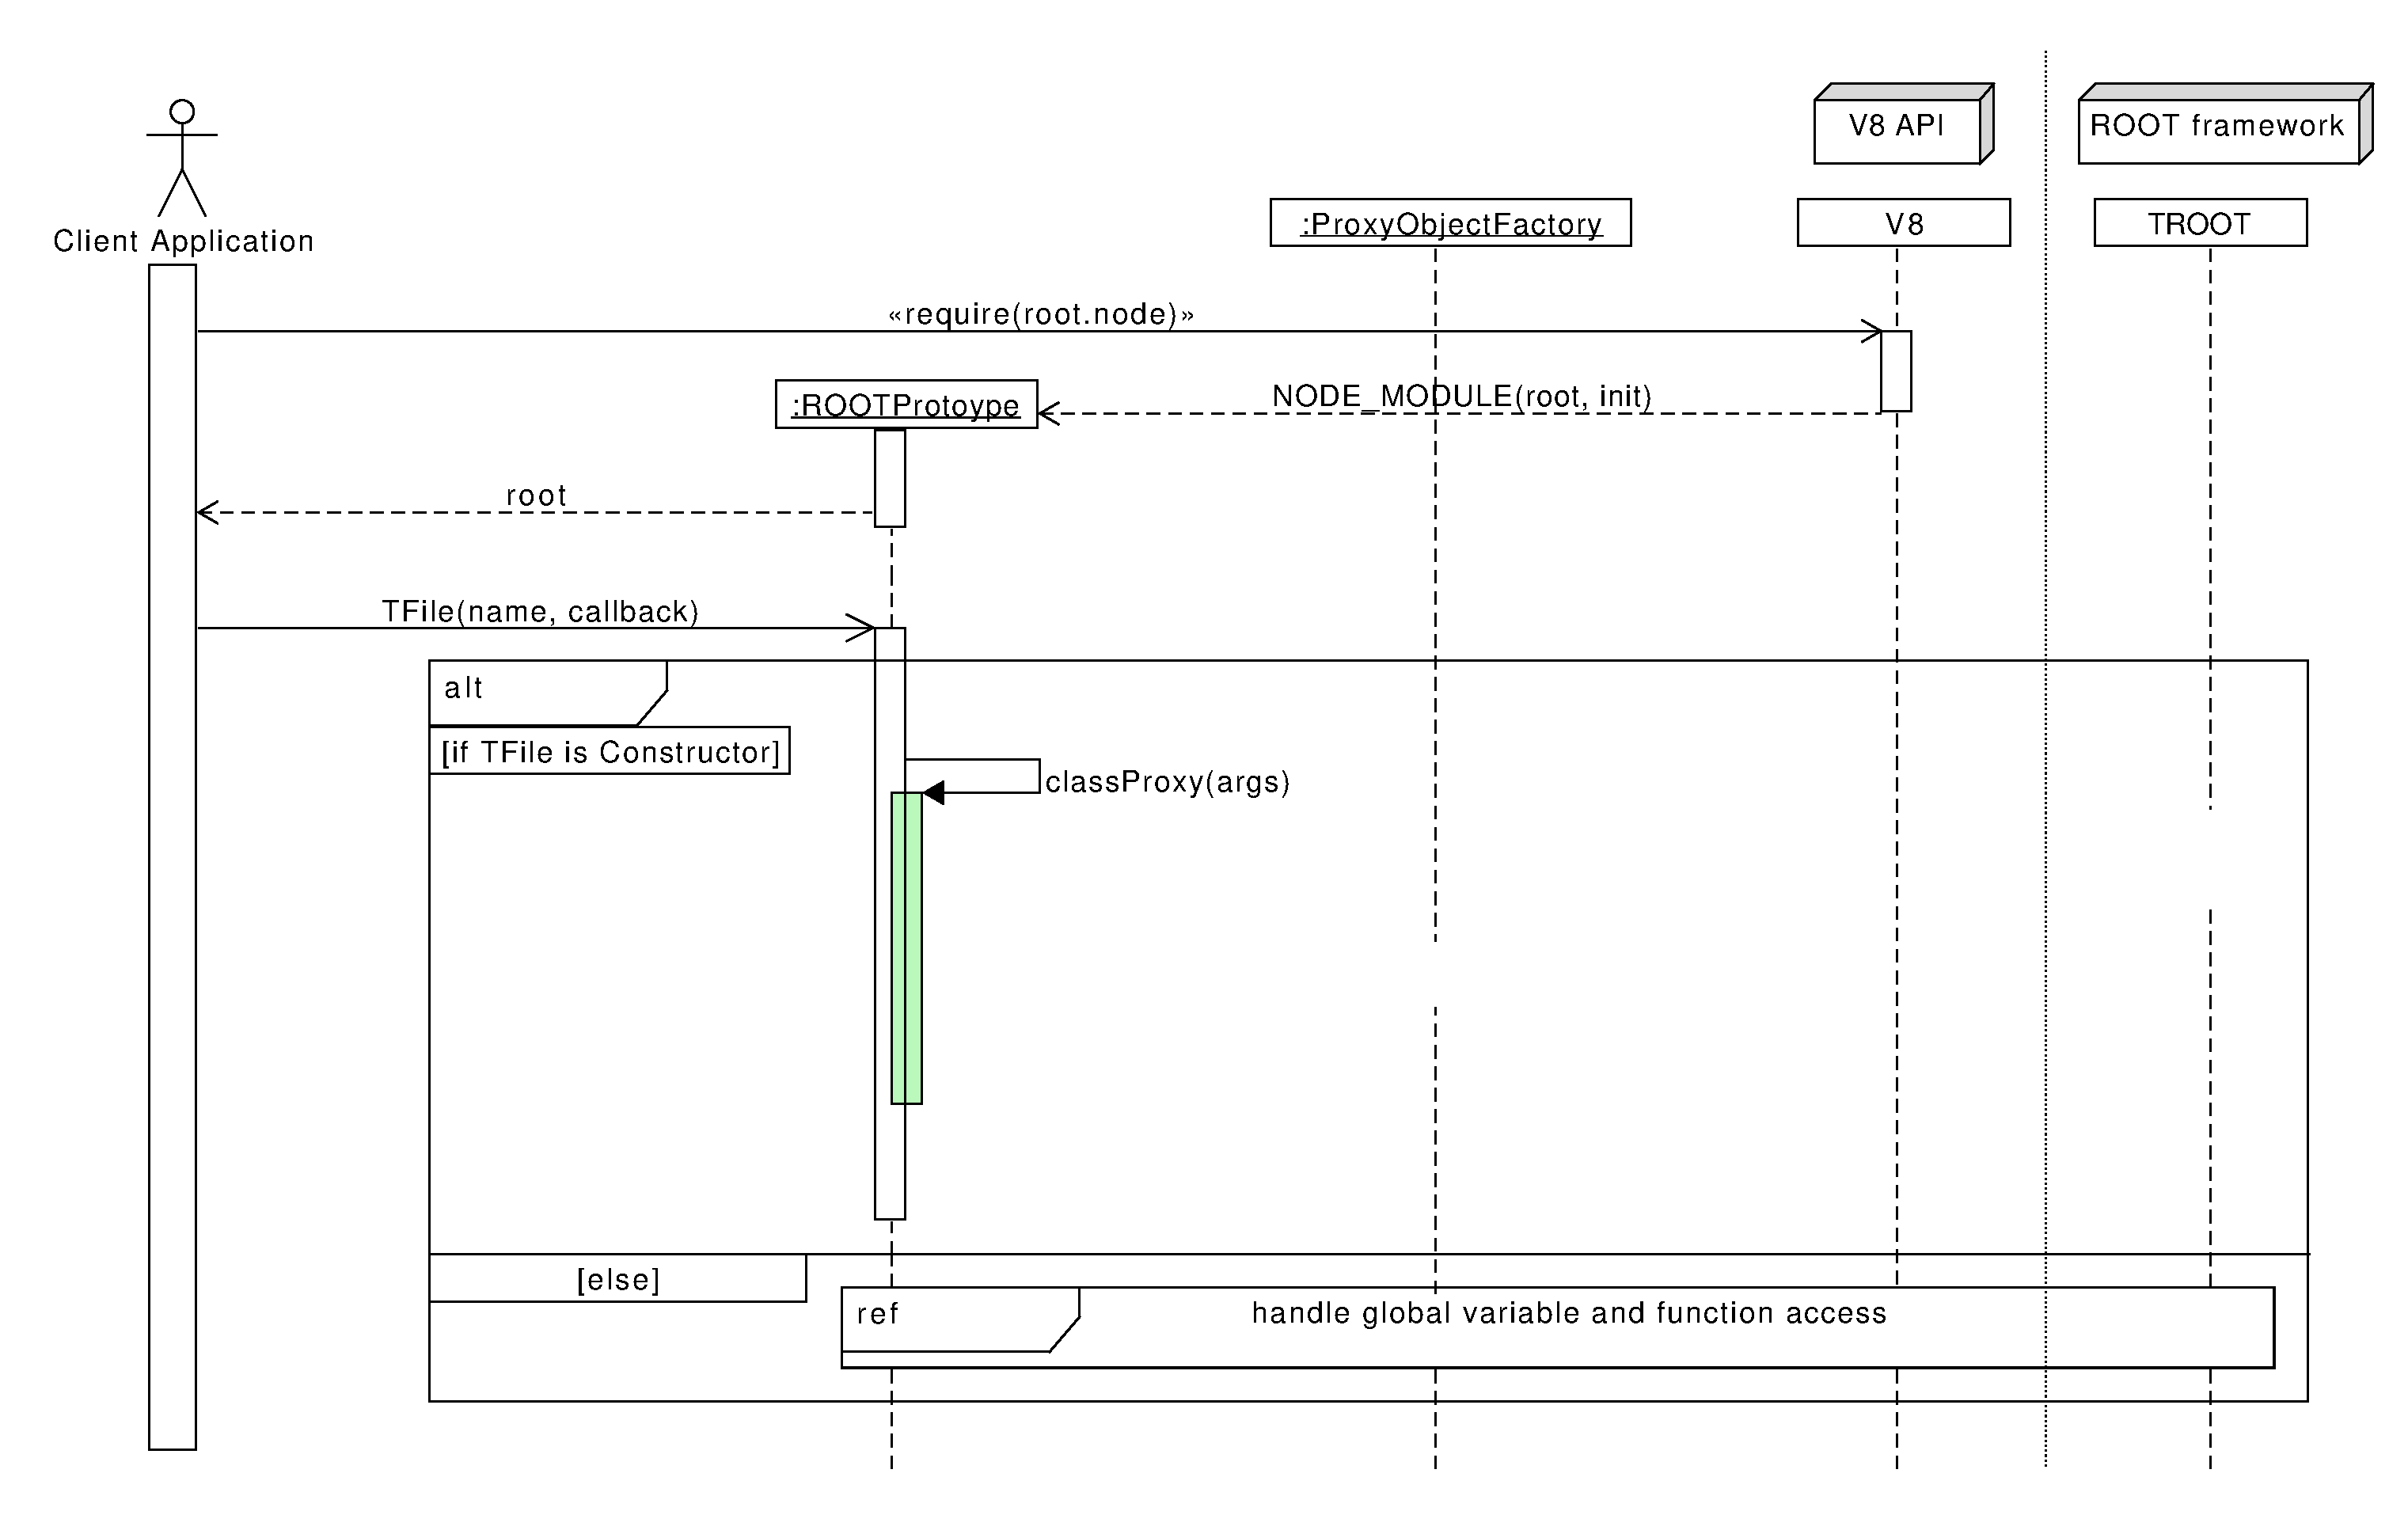
\includegraphics[width=\textwidth, height=.85\textheight, keepaspectratio]{./resources/proxycall/fileOpen_h3.pdf}
  \end{figure}
\end{frame}

\begin{frame}{proxied file access}
  \begin{figure}[htb]
    \centering
      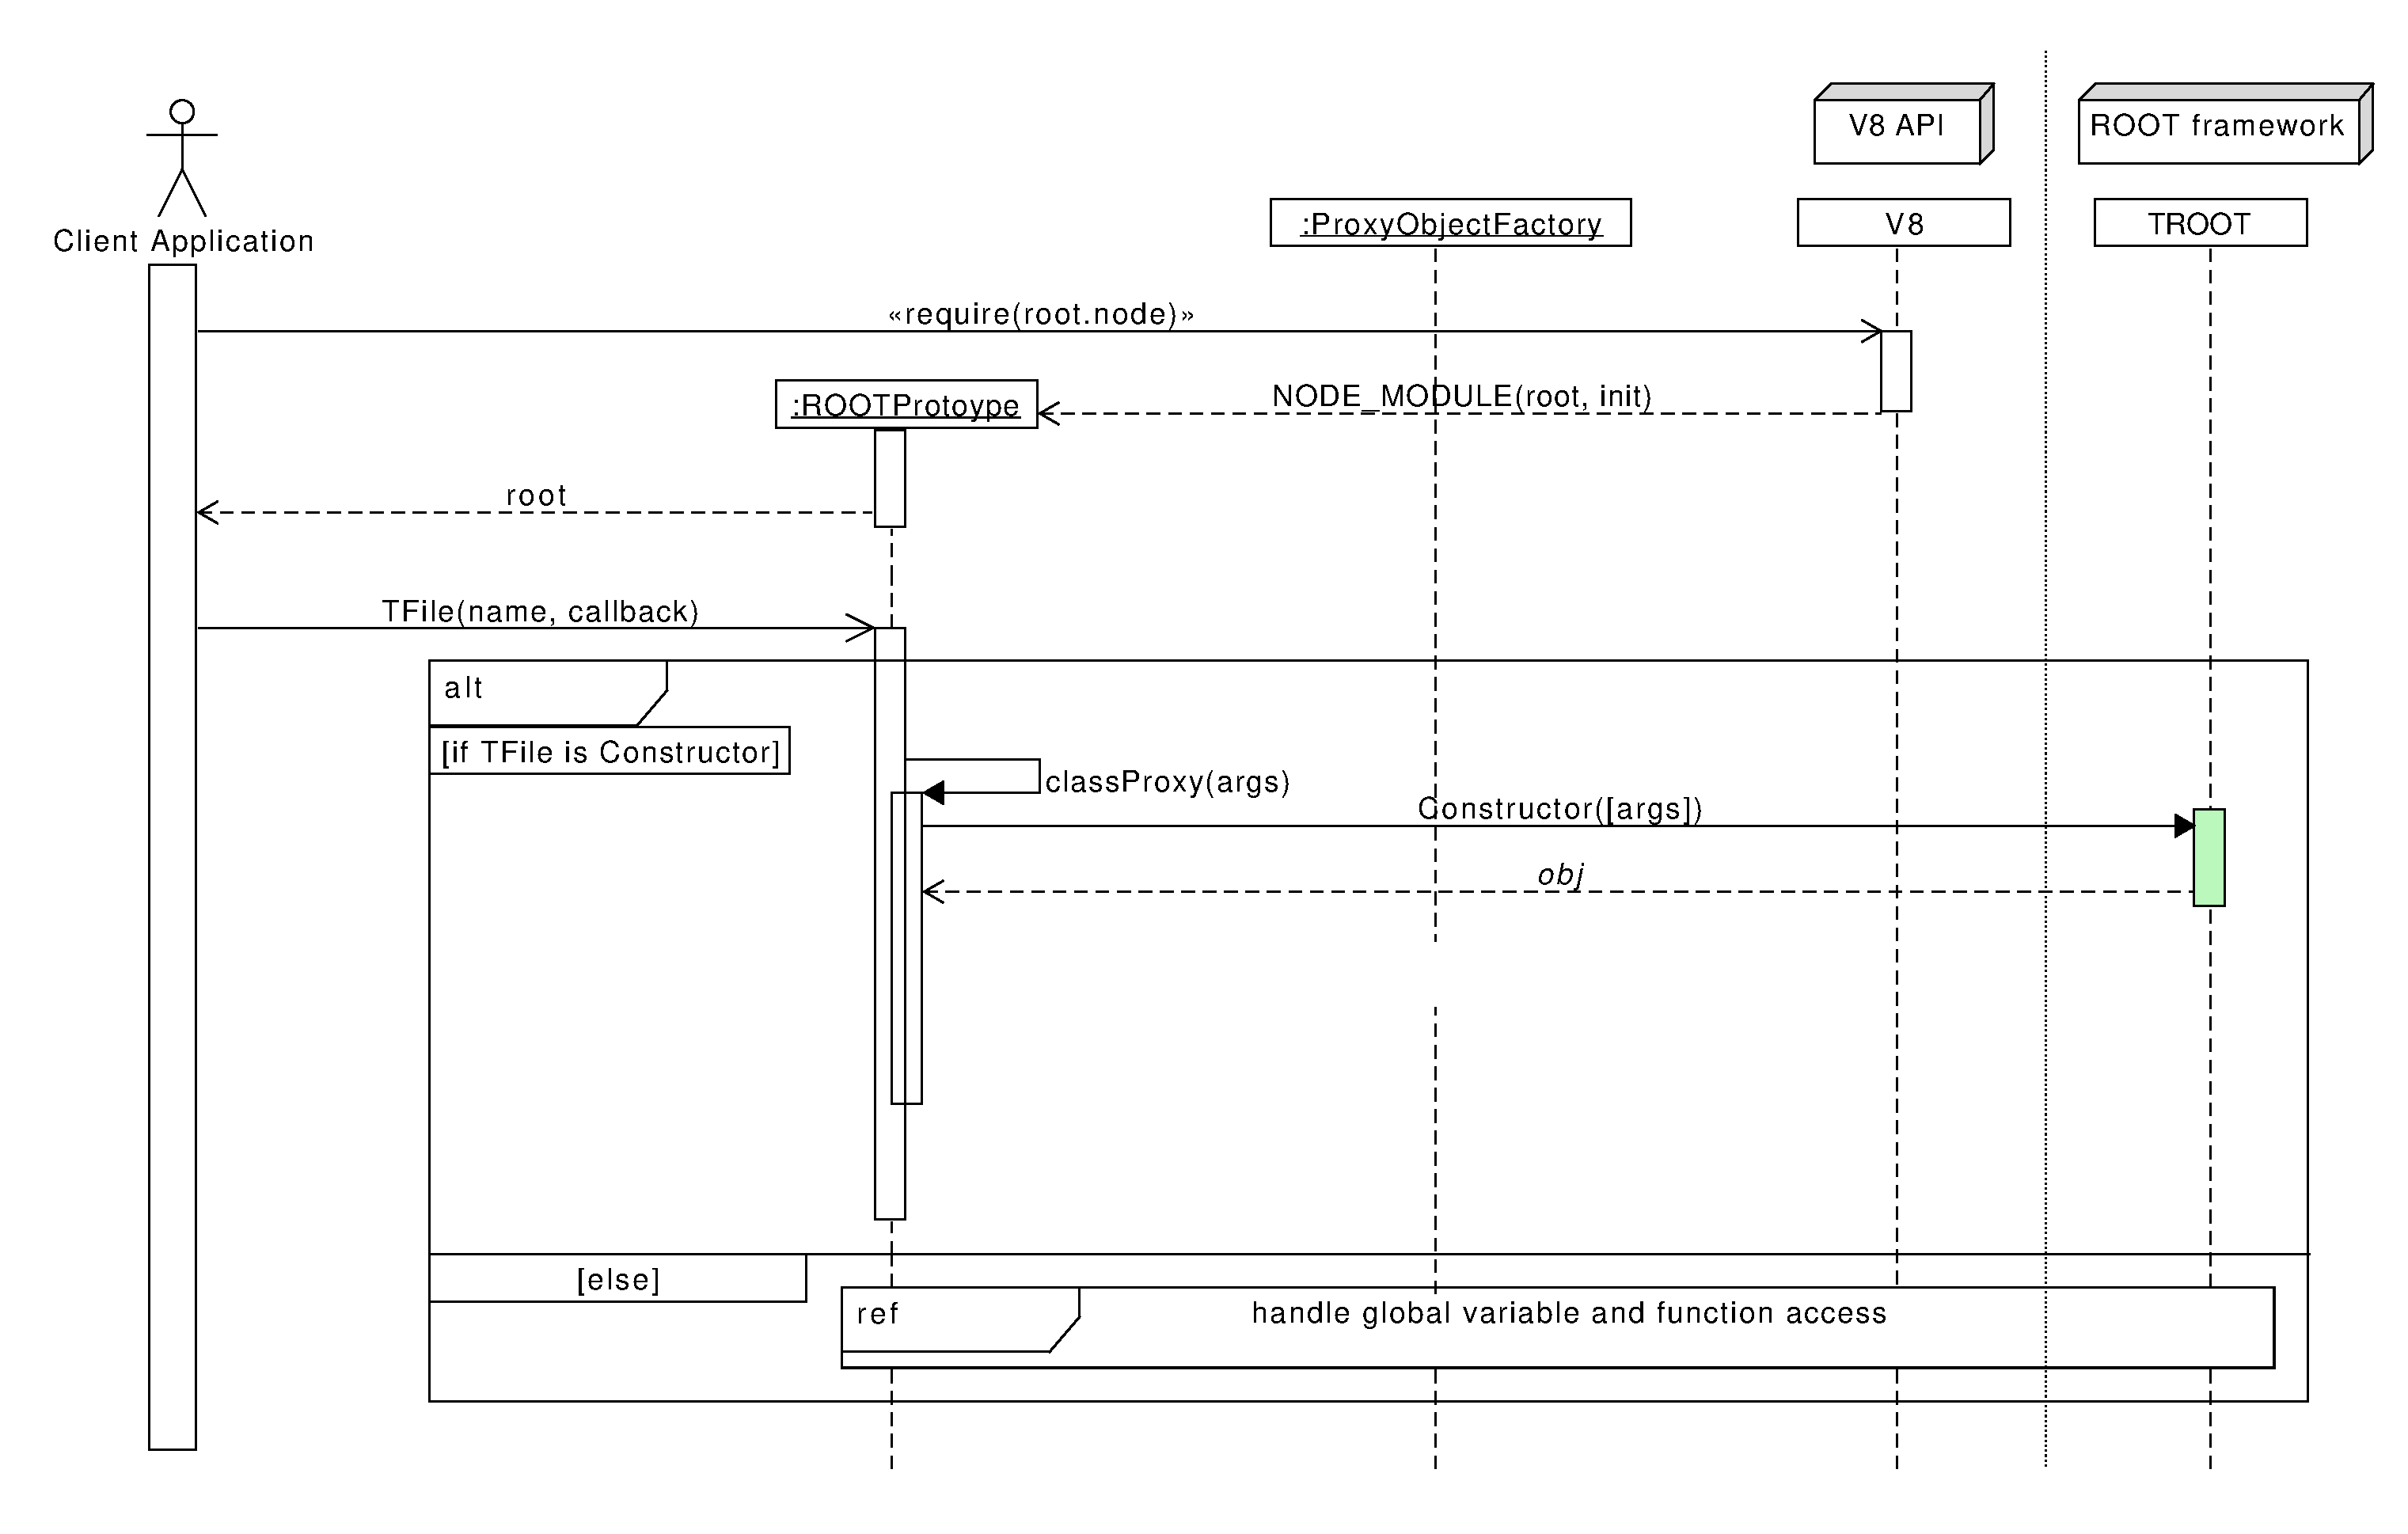
\includegraphics[width=\textwidth, height=.85\textheight, keepaspectratio]{./resources/proxycall/fileOpen_h4.pdf}
  \end{figure}
\end{frame}

\begin{frame}{proxied file access}
  \begin{figure}[htb]
    \centering
      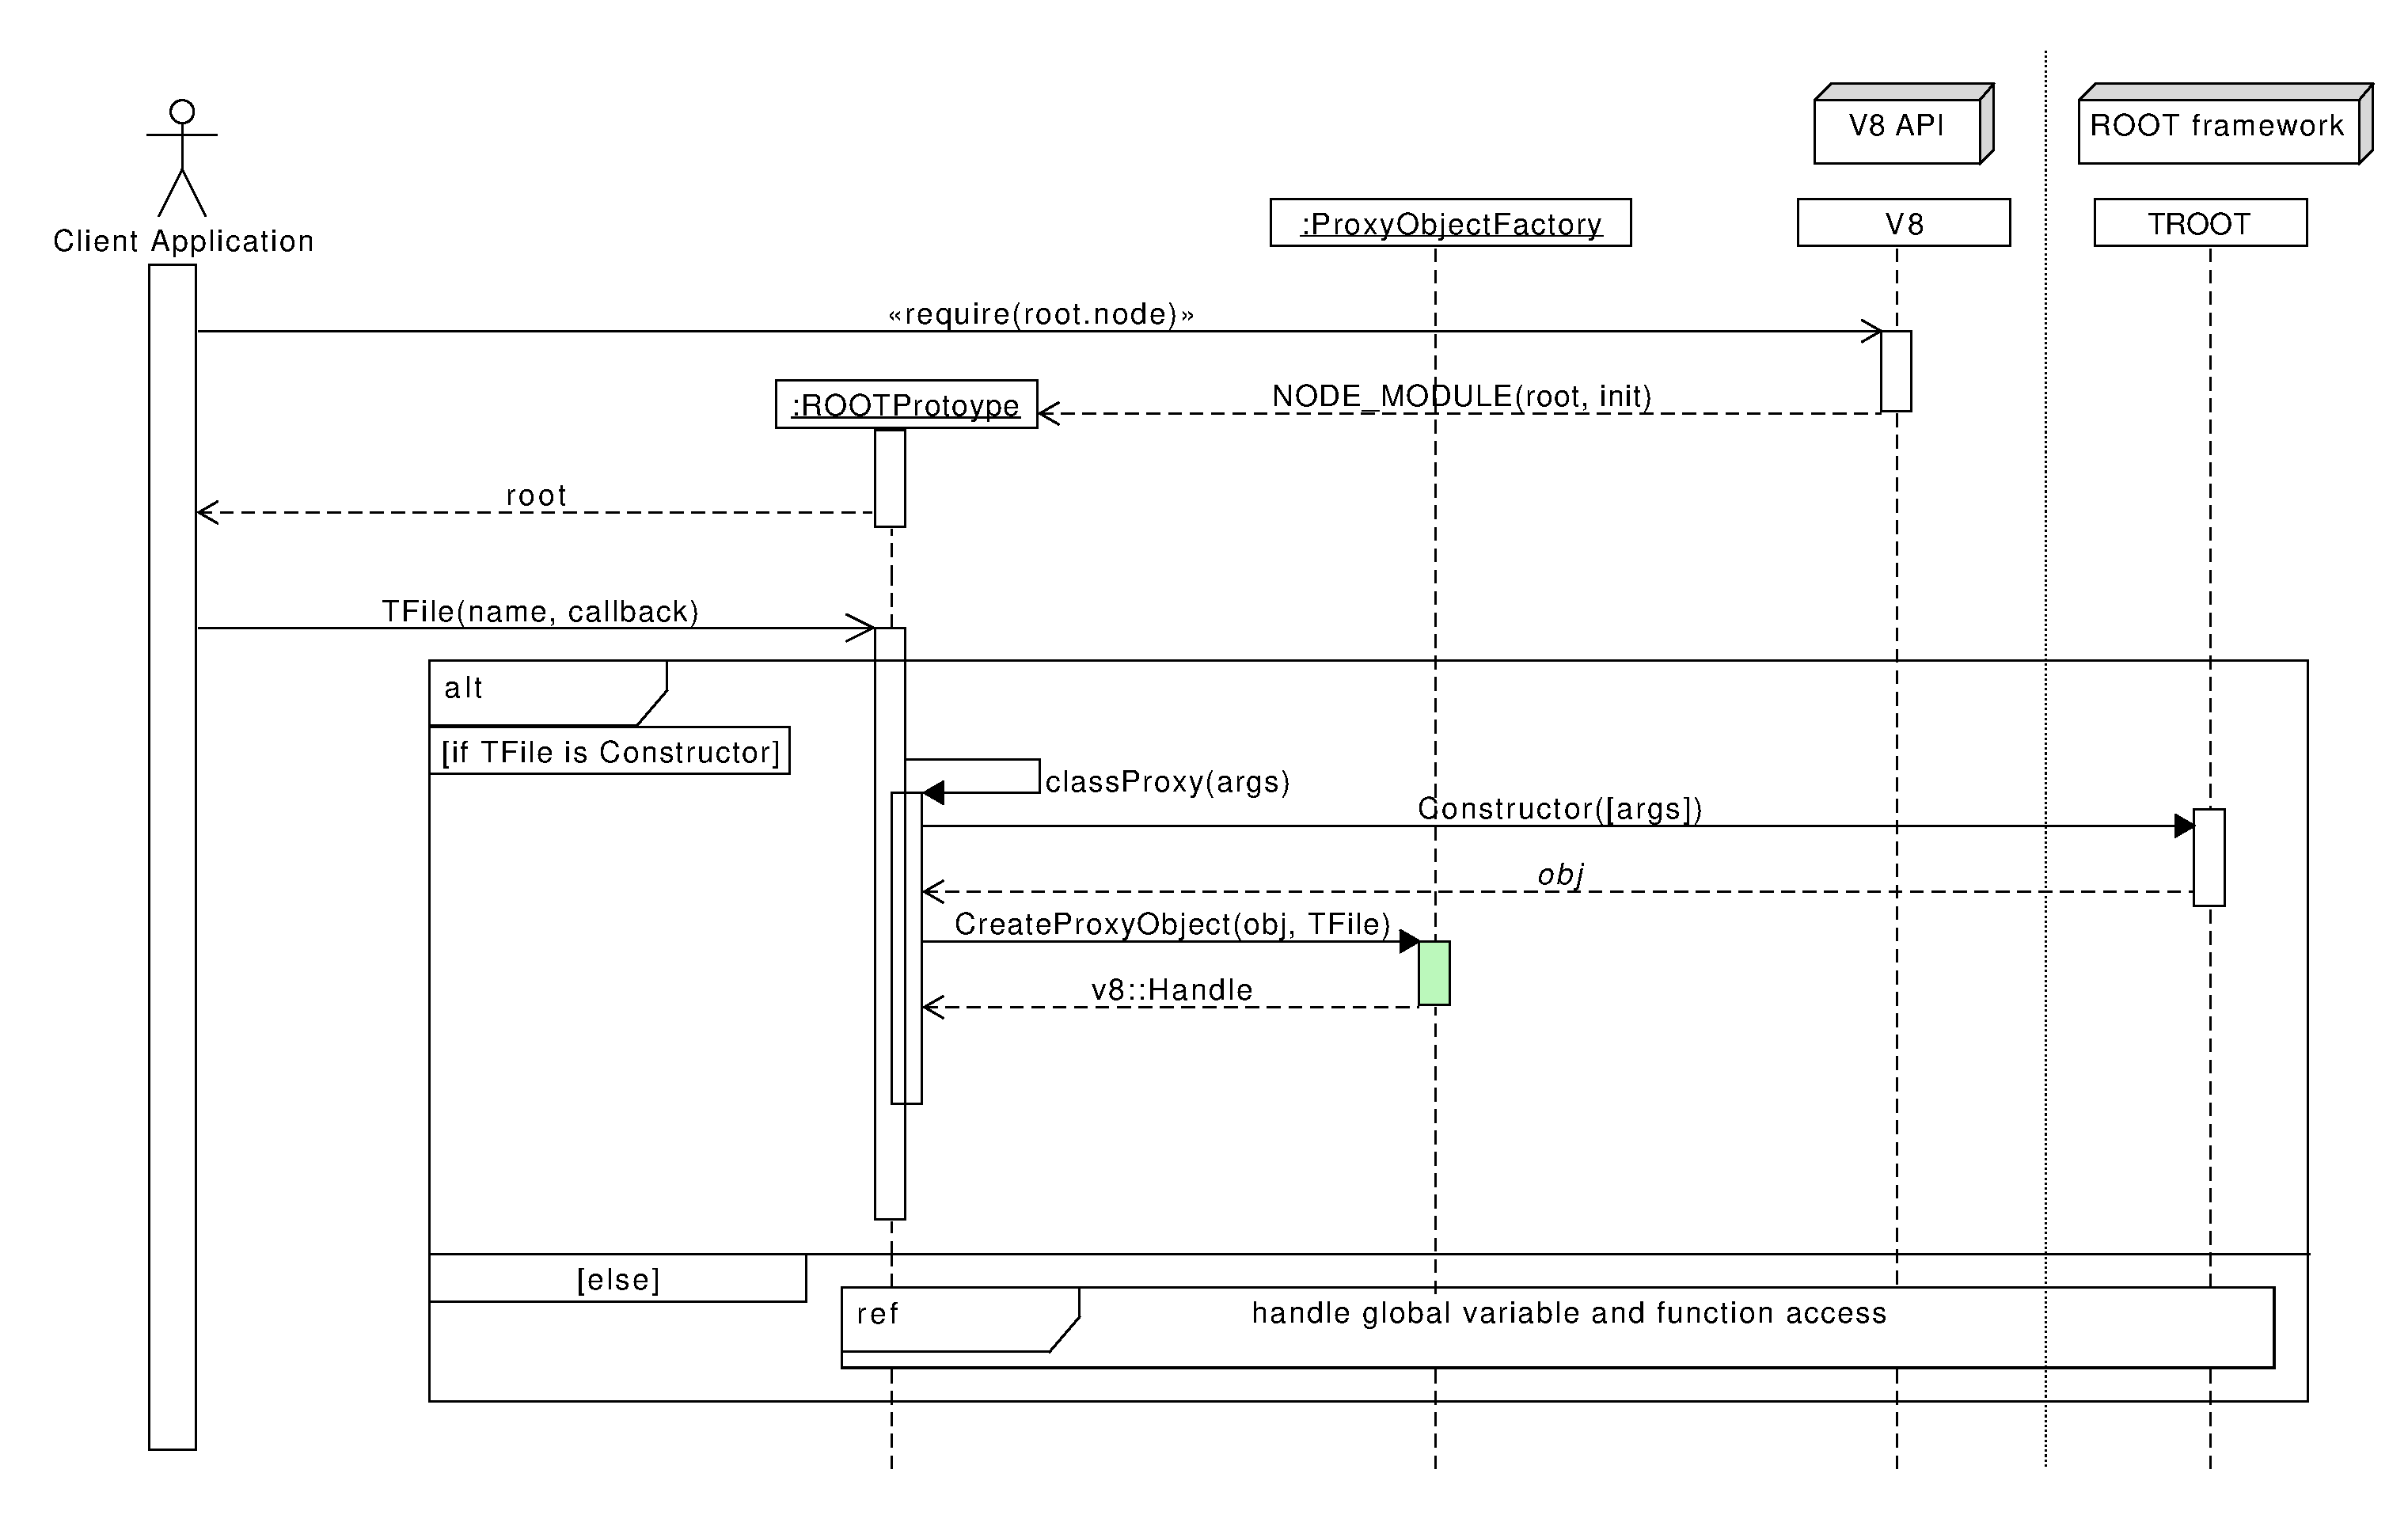
\includegraphics[width=\textwidth, height=.85\textheight, keepaspectratio]{./resources/proxycall/fileOpen_h5.pdf}
  \end{figure}
\end{frame}

\begin{frame}{proxied file access}
  \begin{figure}[htb]
    \centering
      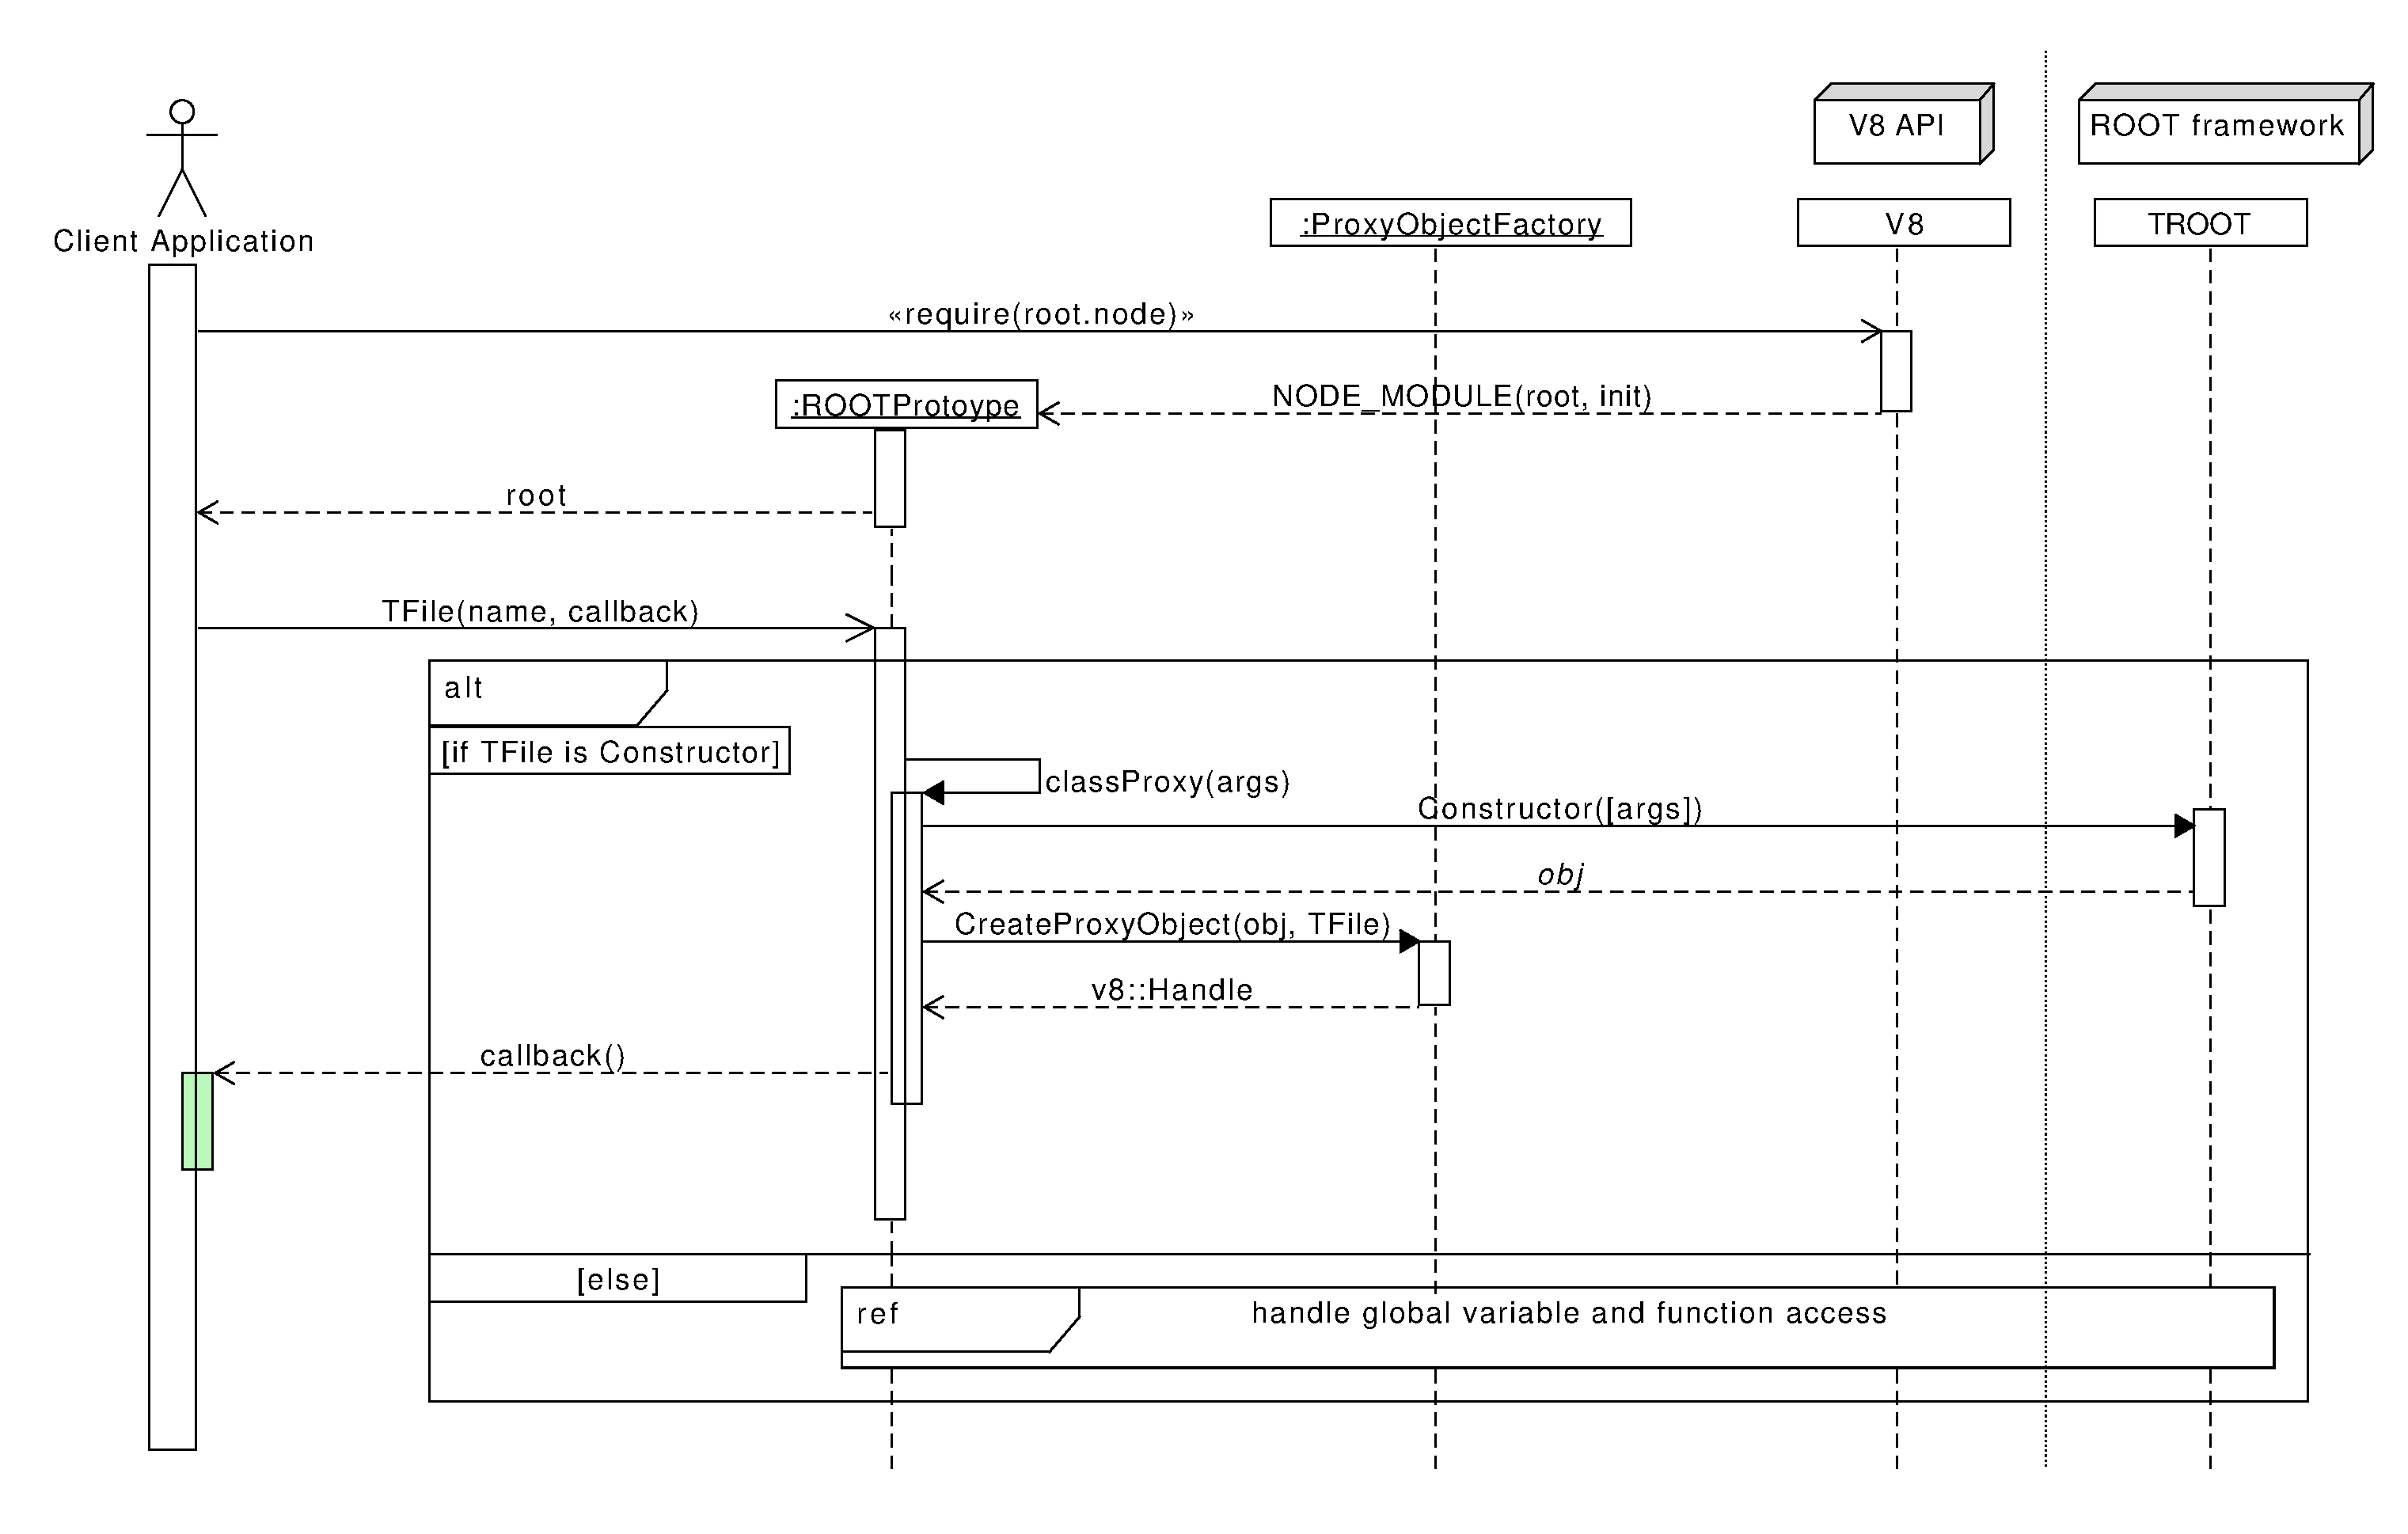
\includegraphics[width=\textwidth, height=.85\textheight, keepaspectratio]{./resources/proxycall/fileOpen_h6.pdf}
  \end{figure}
\end{frame}

\begin{frame}{proxied file access}
  \begin{figure}[htb]
    \centering
      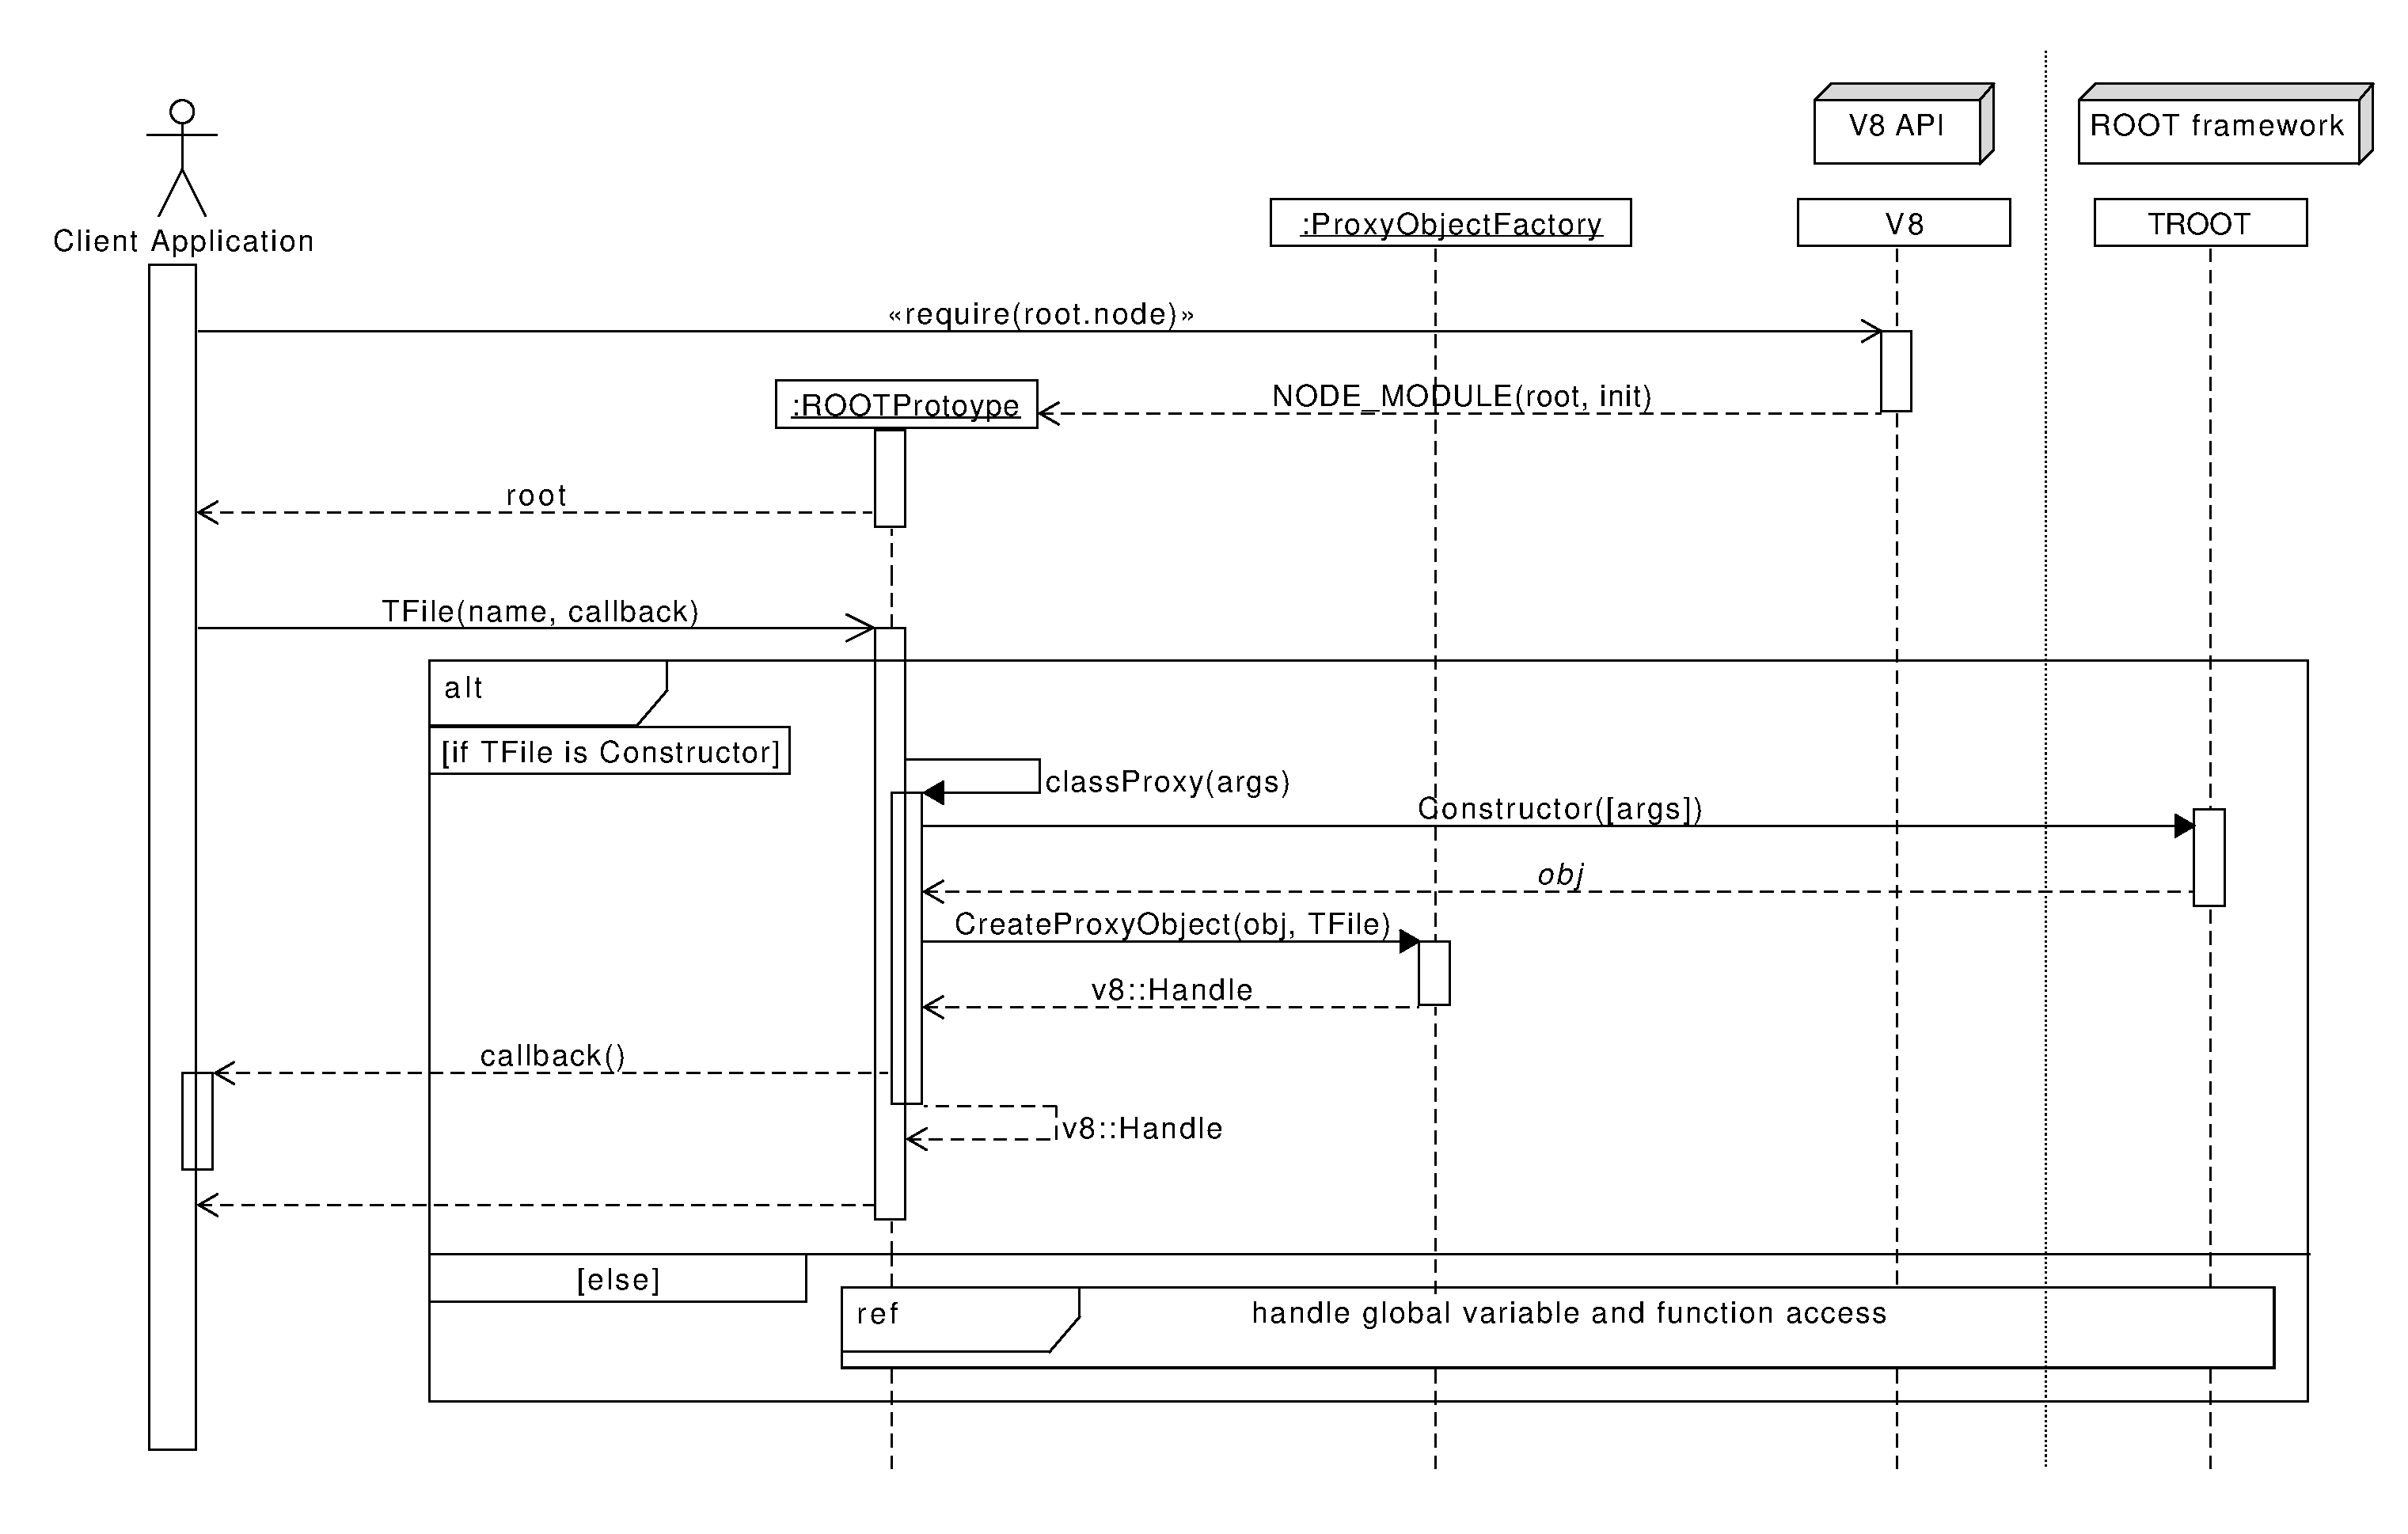
\includegraphics[width=\textwidth, height=.85\textheight, keepaspectratio]{./resources/proxycall/fileOpen_h0.pdf}
  \end{figure}
\end{frame}

